%\documentclass[12pt,serif]{beamer}
%\documentclass[tikz,12pt,svgnames]{beamer}

%For printing (update 2018.12.04: don't use this, handouts doesn't work with my animations option!)
	%\documentclass[table,handout,tikz,12pt,svgnames]{beamer}
%Works with animations option! Change in preamble!
\documentclass[table,tikz,12pt,svgnames]{beamer}

\usepackage{CM-preamble}
\usepackage{gitdags}
\usepackage[compatibility=false]{caption}
\usepackage{subcaption}
%\usepackage{subcaption}
\usepackage{transparent}
\usepackage{eso-pic}
\usepackage{graphicx}
%\usepackage[framemethod=tikz]{mdframed}
\usepackage{mdframed}
\usepackage{lipsum}
\newmdenv[tikzsetting={draw=black,fill=yellow,opacity=0.2, line width=4pt},backgroundcolor=none,leftmargin=0,rightmargin=40,innertopmargin=4pt]{titleBox2}
\newmdenv[leftline=false,rightline=false,topline=false,bottomline=false,tikzsetting={draw=white,fill=white,line width=0pt,},settings={\tikzset{every picture/.style={opacity=0.5}}}]{semiTransparentBox}
\newmdenv[leftline=false,rightline=false,topline=false,bottomline=false,tikzsetting={draw=white,fill=white,line width=0pt,},settings={\tikzset{every picture/.style={opacity=1}}}]{solidBox}
%\newmdenv[tikzsetting={draw=blue,fill=red,},settings={\tikzset{every picture/.style={opacity=0.2}}}]{semiTransparentBox}
\newmdenv[tikzsetting={draw=white,fill=white,line width=0pt,},settings={\tikzset{every picture/.style={opacity=0.2}}}]{titleBox}

\definecolor{darkgreen}{rgb}{0,0.6,0}
\definecolor{red}{rgb}{1,0,0}
\definecolor{green}{rgb}{0,1,0}
\definecolor{blue}{rgb}{0,0,1}
\definecolor{title}{RGB}{51,51,178}
\definecolor{cyan}{rgb}{0.4,1,1}
\definecolor{orange}{rgb}{1,0.7,0}
\definecolor{dkgreen}{rgb}{0,0.6,0}
\definecolor{gray}{rgb}{0.5,0.5,0.5}
\definecolor{purple}{rgb}{0.58,0,0.82}
\definecolor{mintedbackground}{rgb}{0.95,0.95,0.95}
 
\title{\LARGE Gestion de versions}
\subtitle{avec \texttt{git}}
\date{}

\newcommand{\semitransp}[2][35]{\color{fg!#1}#2}


\begin{document}

\begin{frame}
	\titlepage
\end{frame}

%%%%%%%%%%% DÉCHARGE %%%%%%%%%%%
\ifANIMATE
\begin{frame}[noframenumbering]
	\frametitle{Moi... \textit{\small (et ma décharge de responsabilité)}}
	\begin{itemize}
		\item Je suis étranger (hors UE)…
		\item J'ai un accent…
		\item Je me {\color{title} trompe beaucoup} en français
		\begin{itemize}
			\item et en info, et en math, et \ldots
			\item n'hésitez pas à me corriger ou à me demander de répéter
		\end{itemize}
		\item Je commence à enseigner
		\begin{itemize}
			\item ce cours est tout nouveau
			\item j'accepte des critiques (constructives mais pas que)\\
			et surtout des recommandations
			\item n'hésitez pas à poser des questions
		\end{itemize}
		\item Je ne suis pas un expert
	\end{itemize}
\end{frame}
\fi
%%%%%%%%%%%%%%%%%%%%%%%%%%%

\begin{frame}
	\frametitle{Comment gérez-vous vos fichiers ?}
	\vspace{-1em}
	\begin{block}{}
	\begin{itemize}
		\item Garder l'historique
		\item Partager
	\end{itemize}
	\end{block}
	\vspace{-2em}
	\PAUSE
	\begin{block}{}
    \begin{adjustwidth}{-0.5cm}{-0.5cm}{}
		\begin{center}	
		{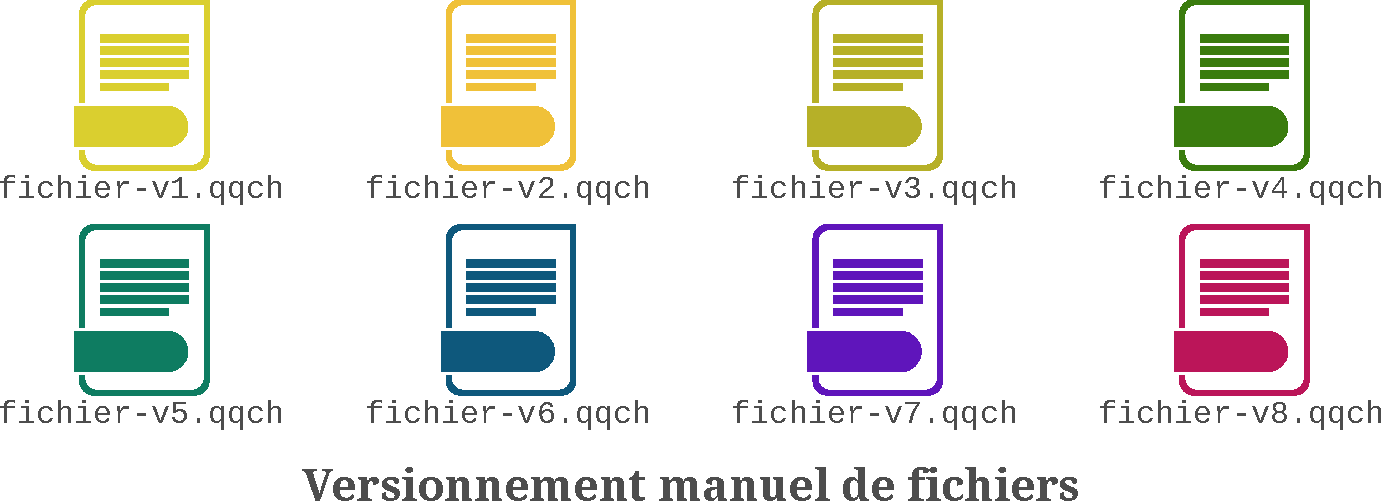
\includegraphics[scale=0.5]{images/file_versions.pdf}}
		\end{center}
	\end{adjustwidth}
	\end{block}
\end{frame}



\begin{frame}
	\frametitle{Comment collaborer sur un fichier ? }
	\vspace{-1em}
	\begin{block}{}
    \begin{adjustwidth}{-0.5cm}{-0.5cm}{}
		\begin{center}
		{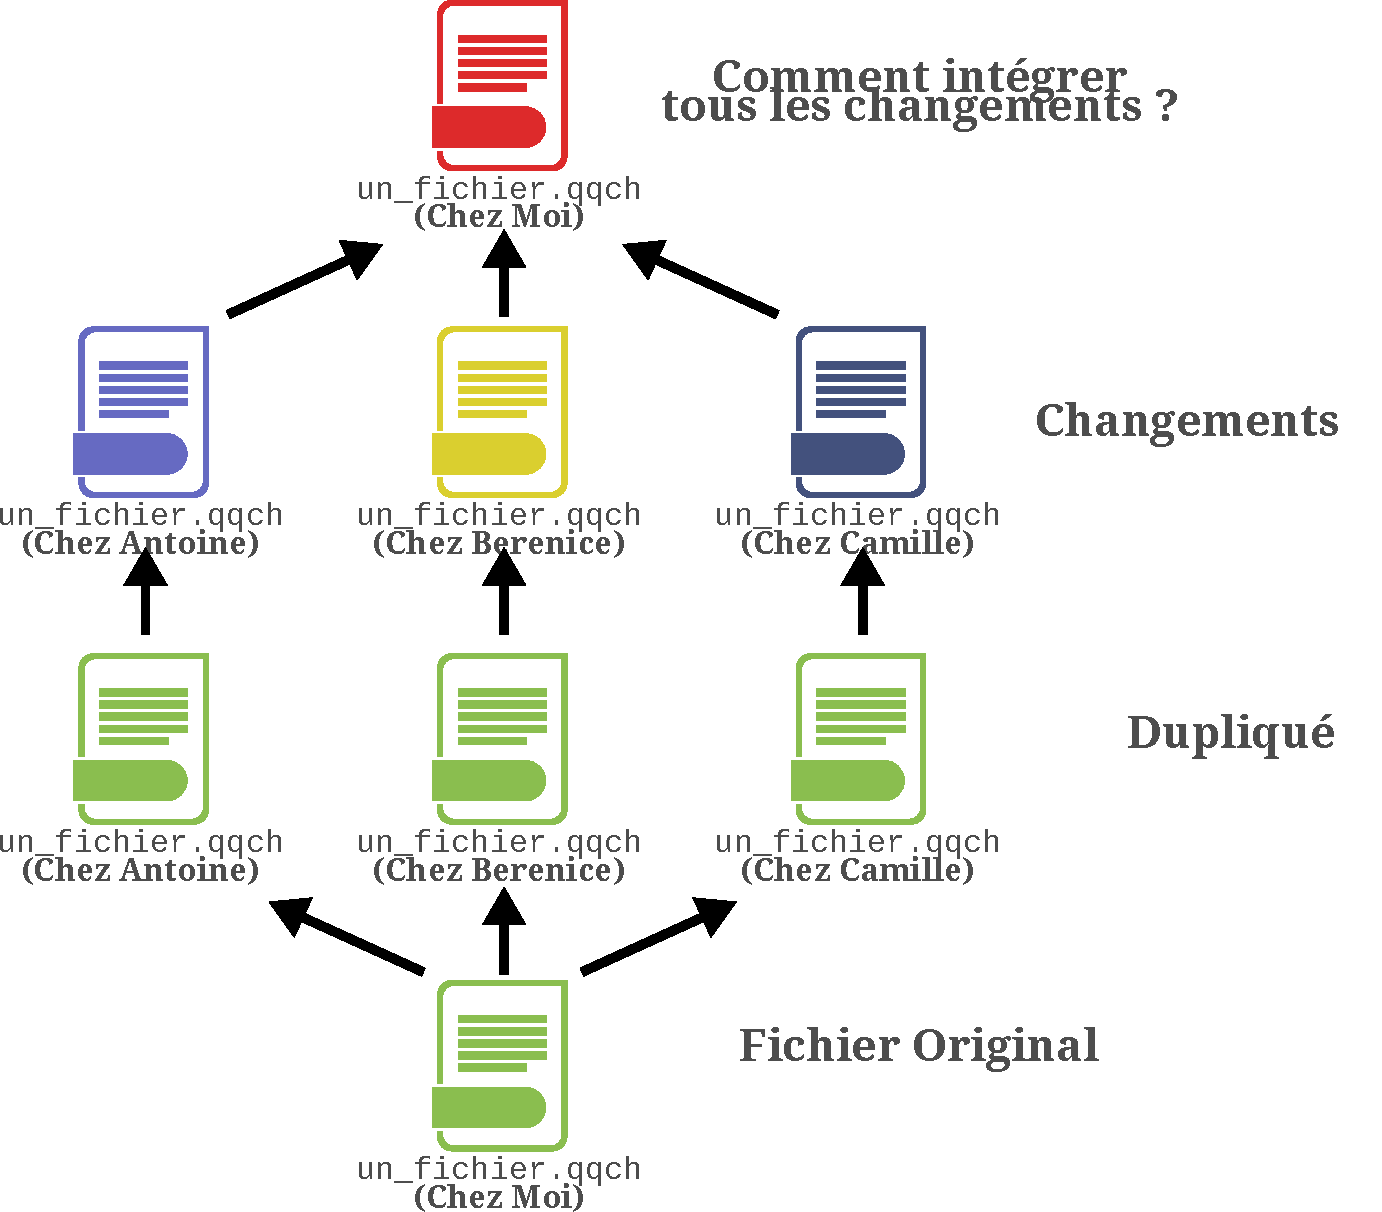
\includegraphics[scale=0.38]{images/file_share.pdf}}
		\end{center}
	\end{adjustwidth}
	\end{block}
\end{frame}


\begin{frame}
	\frametitle{Comment collaborer sur \underline{plusieurs} fichiers ? }
%	\vspace{-4em}
	\begin{block}{}
    \begin{adjustwidth}{-0.5cm}{-0.5cm}{}
		\begin{center}
		{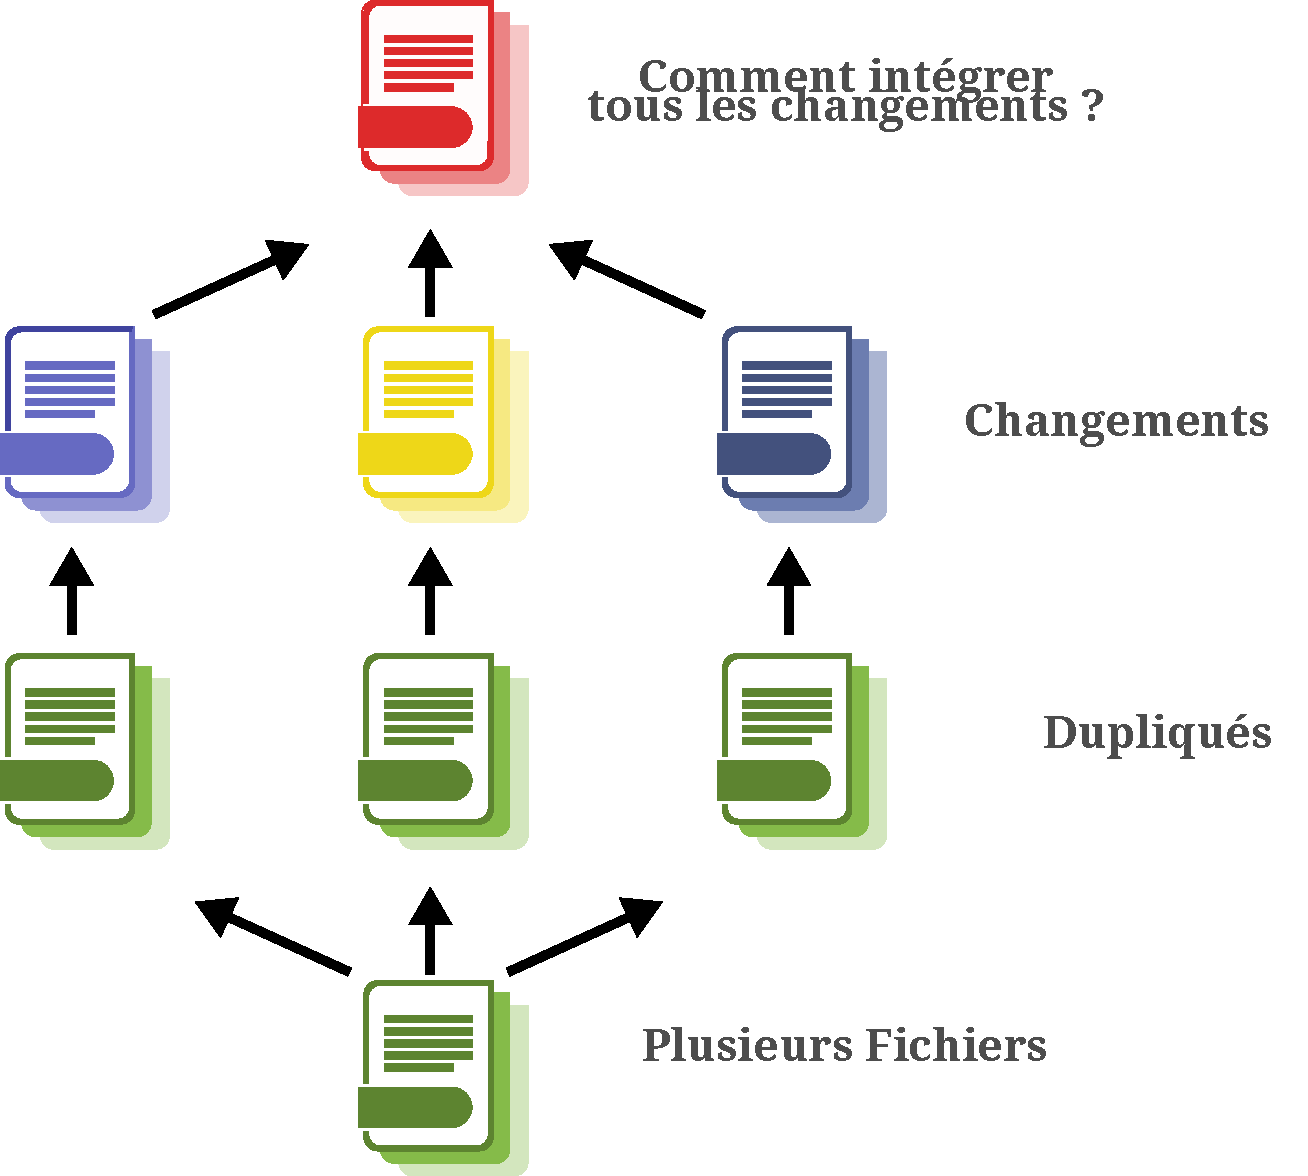
\includegraphics[scale=0.38]{images/file_share_many.pdf}}
		\end{center}
	\end{adjustwidth}
	\end{block}
\end{frame}


\begin{frame}
	\frametitle{D'autres solutions ? }
	\vspace{-4em}
	\begin{block}{}
    \begin{adjustwidth}{-0.5cm}{-0.5cm}{}
		\begin{center}
		{
\includegraphics[scale=0.43]{images/services.pdf}}
		\end{center}
	\end{adjustwidth}
	\end{block}
\end{frame}

\begin{frame}
	\frametitle{Problématique : développement logiciel}
	\begin{block}{}
    \begin{adjustwidth}{-0.3cm}{-1.4cm}{}
		\begin{itemize}
			\item Un \textcolor{title}{projet} de développement logiciel est une activité longue et
			complexe.
			\item Concerne plusieurs \textcolor{title}{fichiers} (milliers !)
			\item De multiples \textcolor{title}{itérations} sont nécessaires.
			\item A certains moments, on peut identifier des \textcolor{title}{versions} et/ou \textcolor{title}{variantes} du logiciel.
			\item Les erreurs sont possibles, \textcolor{title}{revenir en arrière} est parfois nécessaire.
			\item Un projet peut se faire à plusieurs, les développeurs peuvent travailler sur les mêmes fichiers (\textcolor{title}{conflits})
		\end{itemize}
	\end{adjustwidth}
	\end{block}
\end{frame}

\begin{frame}
	\frametitle{Définitions}
		\begin{block}{Simple}
			\begin{itemize}
				\item Un \textbf{gestionnaire de versions} est un logiciel qui \textbf{enregistre les évolutions d’un ensemble de fichiers} au cours du temps de manière à ce qu'on puisse rappeler une version antérieure à̀ tout moment.
			\end{itemize}
		\end{block}
		\begin{block}{Définition Wikipedia\footnote{\url{https://fr.wikipedia.org/wiki/Gestion\_de\_versions}}}
			\begin{itemize}
				\item La \textbf{gestion de versions} (en anglais \textit{version control} ou \textit{revision control}) consiste à maintenir \textbf{l'ensemble des versions d'un ou plusieurs fichiers} (généralement en texte).
				Essentiellement utilisée dans le domaine de la création de logiciels, elle concerne surtout \textbf{la gestion des codes source}.
			\end{itemize}
		\end{block}
\end{frame}


\begin{frame}
	\frametitle{Gestion de versions}
	\vspace{-2.7em}
	\begin{block}{}
%    \begin{adjustwidth}{-5.5cm}{-0.5cm}{}
		\small Le développement logiciel est un processus sinueux à notion de \textcolor{title}{branche} (chaque noeud représente un \textcolor{title}{ensemble de fichiers} à un temps $t$) :
		\vspace{-1em}
		\begin{center}
		{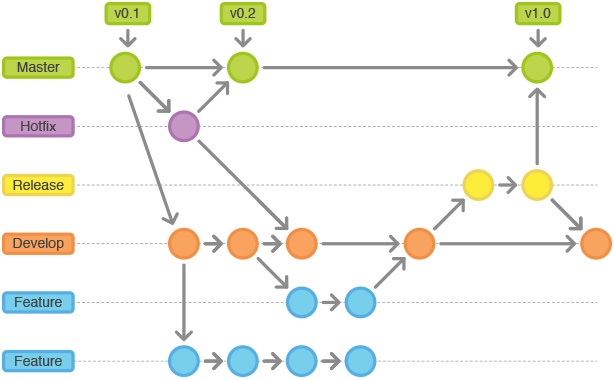
\includegraphics[scale=0.48]{images/git_flow.png}}
		\end{center}
%	\end{adjustwidth}
	\vspace{-4em}
%    \begin{adjustwidth}{5.0cm}{-1.5cm}{}
%	\tiny Par Revision\_controlled\_project\_visualization.svg: *Subversion\_project\_visualization.svg: Traced by User:Stannered, original by en:User:Sami Keroladerivative work: Moxfyre (talk)derivative work: Echion2 (talk) — Revision\_controlled\_project\_visualization.svg, CC BY-SA 3.0, \url{https://commons.wikimedia.org/w/index.php?curid=9562807}
%	\end{adjustwidth}
	\end{block}
\end{frame}

%%%%%%%%%%%%%%%%%%%%%%%%%%%%%%%%%%%%%%%%%%%%%%%%%%%%% BEGIN OLD GESTION VERSIONS
%\begin{frame}
%	\frametitle{Gestion de versions}
%	\vspace{-2em}
%	\begin{block}{}
%    \begin{adjustwidth}{-5.5cm}{-0.5cm}{}
%		\begin{center}
%		{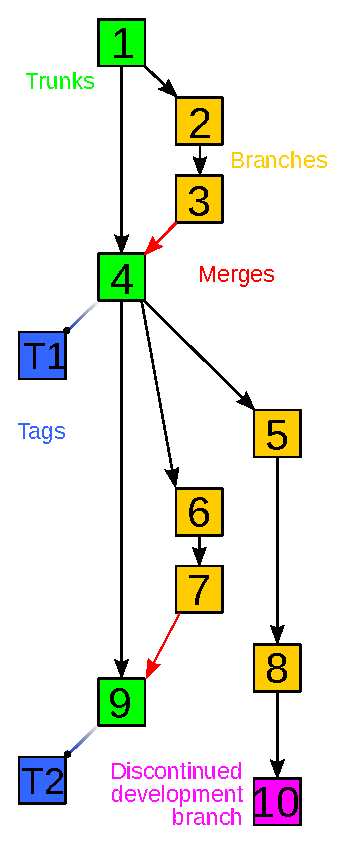
\includegraphics[scale=0.58]{images/gestion_versions.pdf}}
%		\end{center}
%	\end{adjustwidth}
%	\vspace{-4em}
%    \begin{adjustwidth}{5.0cm}{-1.5cm}{}
%	\tiny Par Revision\_controlled\_project\_visualization.svg: *Subversion\_project\_visualization.svg: Traced by User:Stannered, original by en:User:Sami Keroladerivative work: Moxfyre (talk)derivative work: Echion2 (talk) — Revision\_controlled\_project\_visualization.svg, CC BY-SA 3.0, \url{https://commons.wikimedia.org/w/index.php?curid=9562807}
%	\end{adjustwidth}
%	\end{block}
%\end{frame}
%
%\begin{frame}
%	\frametitle{Gestion de versions}
%		\begin{block}{}
%				La \textbf{gestion de versions} (en anglais \textit{version control} ou \textit{revision control}) consiste à maintenir \textbf{l'ensemble des versions d'un ou plusieurs fichiers} (généralement en texte).
%				Essentiellement utilisée dans le domaine de la création de logiciels, elle concerne surtout \textbf{la gestion des codes source}.
%		\end{block}
%		\begin{block}{}
%		\small \url{https://fr.wikipedia.org/wiki/Gestion\_de\_versions}
%		\end{block}
%\end{frame}
%%%%%%%%%%%%%%%%%%%%%%%%%%%%%%%%%%%%%%%%%%%%%%%%%%%%% END OLD GESTION VERSIONS

\begin{frame}
	\frametitle{Avantages de la gestion de versions}
	\begin{block}{}
    \begin{adjustwidth}{-0.3cm}{-1.4cm}{}
		\begin{itemize}
			\item Sauvegarde / Restauration
			\item Synchronisation du travail (partage, collaboration)
			\item Suivi de changements (très détaillé)
			\item Suivi de responsabilités / propriétaires / coupables
			\item \textit{Sandboxing} (espace confiné, environnement de test, isolation)
			\item \textit{Branching and merging}
			\item Passage à l'échelle (10, 100, 1.000, 10.000 développeurs)
		\end{itemize}
	\end{adjustwidth}
	\end{block}
\end{frame}

\begin{frame}
	\frametitle{Que mettre dans un Logiciel de Gestion de Versions ?}
	\vspace{-2em}
	\begin{block}{}%À mettre
    \begin{adjustwidth}{-0.5cm}{}
		\begin{itemize}
			\item Tous les sources du projet
			\begin{itemize}
				\item code source (\texttt{.c .cpp .java .py} \dots)
				\item scripts de build (\texttt{Makefile pom.xml} \ldots)
				\item Documentation (\texttt{.txt .tex Readme} \ldots)
				\item Ressources (images \ldots)
				\item Scripts divers (déploiement, \texttt{.sql, .sh} \ldots)
			\end{itemize}
		\end{itemize}
	\end{adjustwidth}	
	\end{block}
	\PAUSE
	\begin{block}{\color{red} \underline{\textbf{À NE PAS METTRE}}}
    \begin{adjustwidth}{-0.5cm}{}
	\begin{itemize}
		\item Les fichiers générés
		\begin{itemize}
			\item Résultat de compilation (\texttt{.class .o .exe .jar} \ldots)
			\item Autres fichiers générés (\texttt{.ps .dvi .pdf javadoc} \ldots)
		\end{itemize}
	\end{itemize}
	\end{adjustwidth}
	\end{block}
\end{frame}

\begin{frame}
\frametitle{Why \textit{the \texttt{git}} ?}
\begin{block}{C'est \textit{Ze Standard}}
	%    \begin{adjustwidth}{-0.9cm}{}
	\begin{itemize}
		\item \textit{git - the stupid content tracker}
		\item Linus Torvalds (2005)
		\item Outil professionnel, rapide, multi-plateforme, flexible, puissant, complètement distribué
	\end{itemize}
%	\end{adjustwidth}
\end{block}
\begin{block}{\textit{To Share or Not to Share ?}}
	\begin{itemize}
		\item Enrichissez vos CV
		\begin{itemize}
			\item Faites un compte sur \url{https://github.com/}
		\end{itemize}
		\item Choisir sa licence
		\begin{itemize}
			\item Code --- GPL, Apache, BSD, MIT, Propriétaire \url{https://choosealicense.com/}
			\item Documents/Rapports --- Creative commons \url{https://creativecommons.org/}
		\end{itemize}
	\end{itemize}
\end{block}
\end{frame}

\newcounter{numSlide}

\begin{frame}
\frametitle{Concepts et commandes \texttt{git}}
\begin{adjustwidth}{-0.75cm}{0cm}{}
\vspace{-1em}
	\begin{center}
		\setcounter{numSlide}{1}
		\ifANIMATE
			\only<\value{numSlide}>{{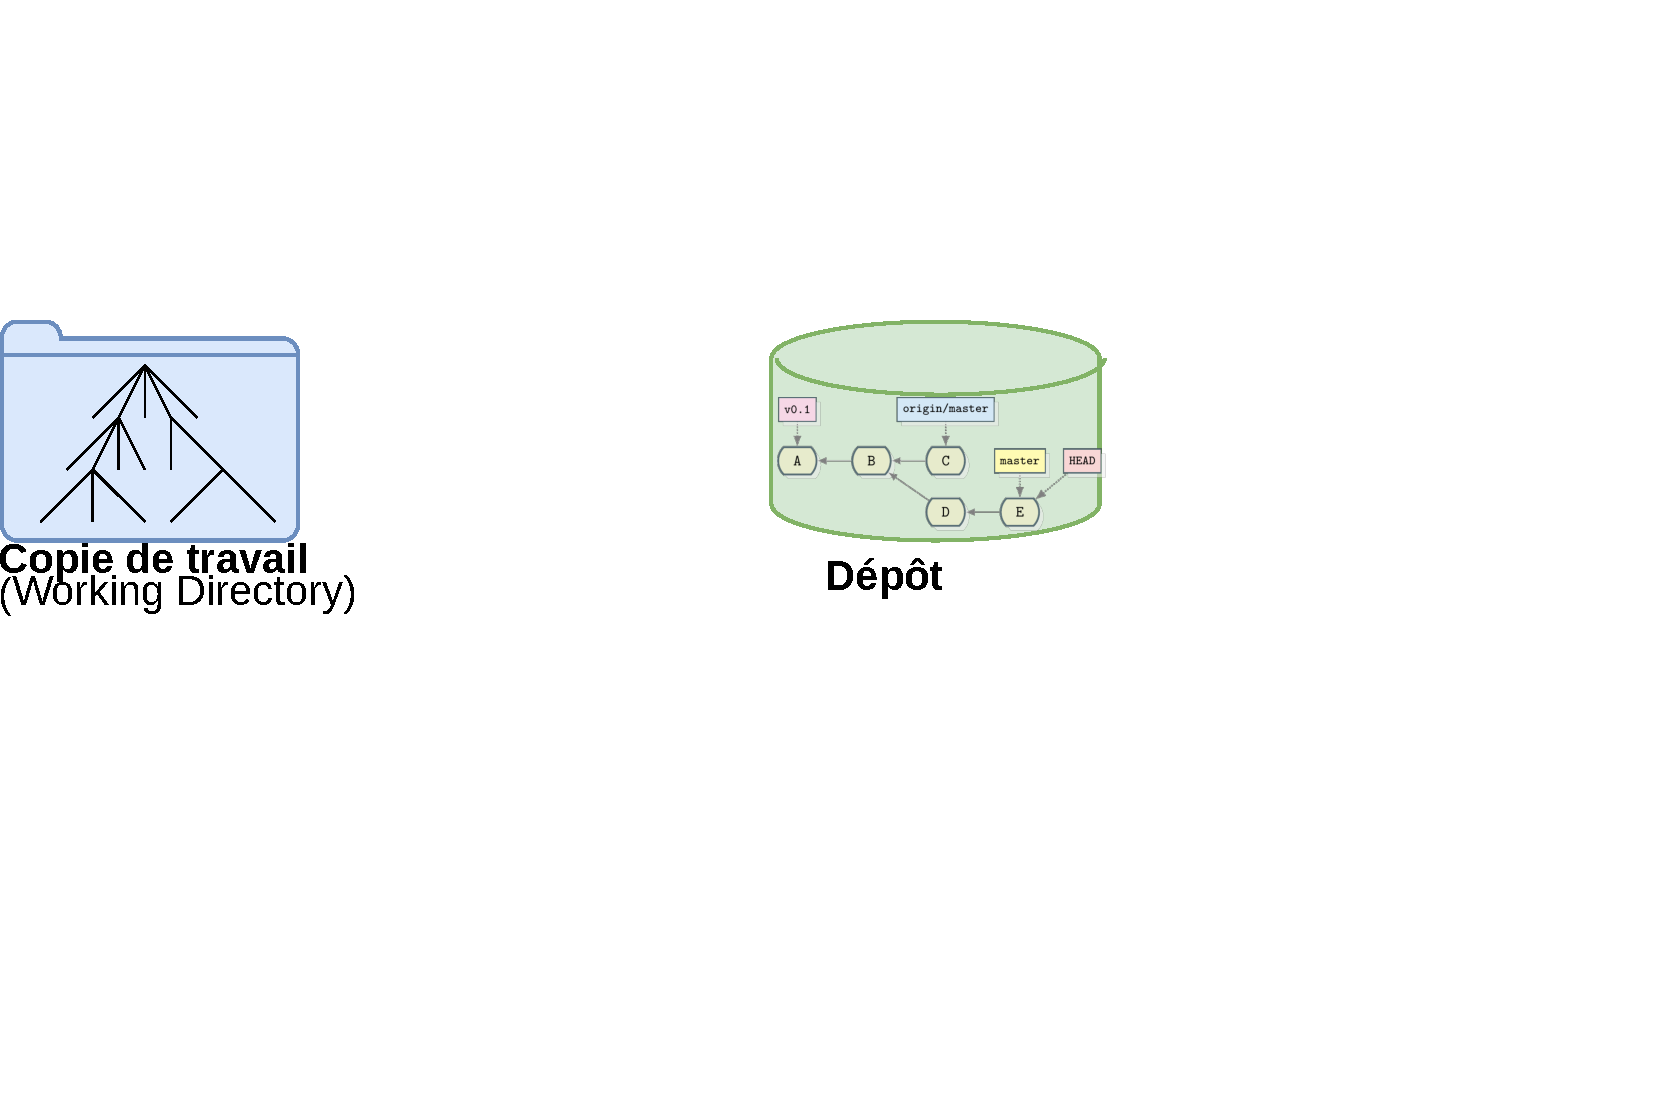
\includegraphics[scale=0.44]{images/workflow1.pdf}}}\stepcounter{numSlide}
			\only<\value{numSlide}>{{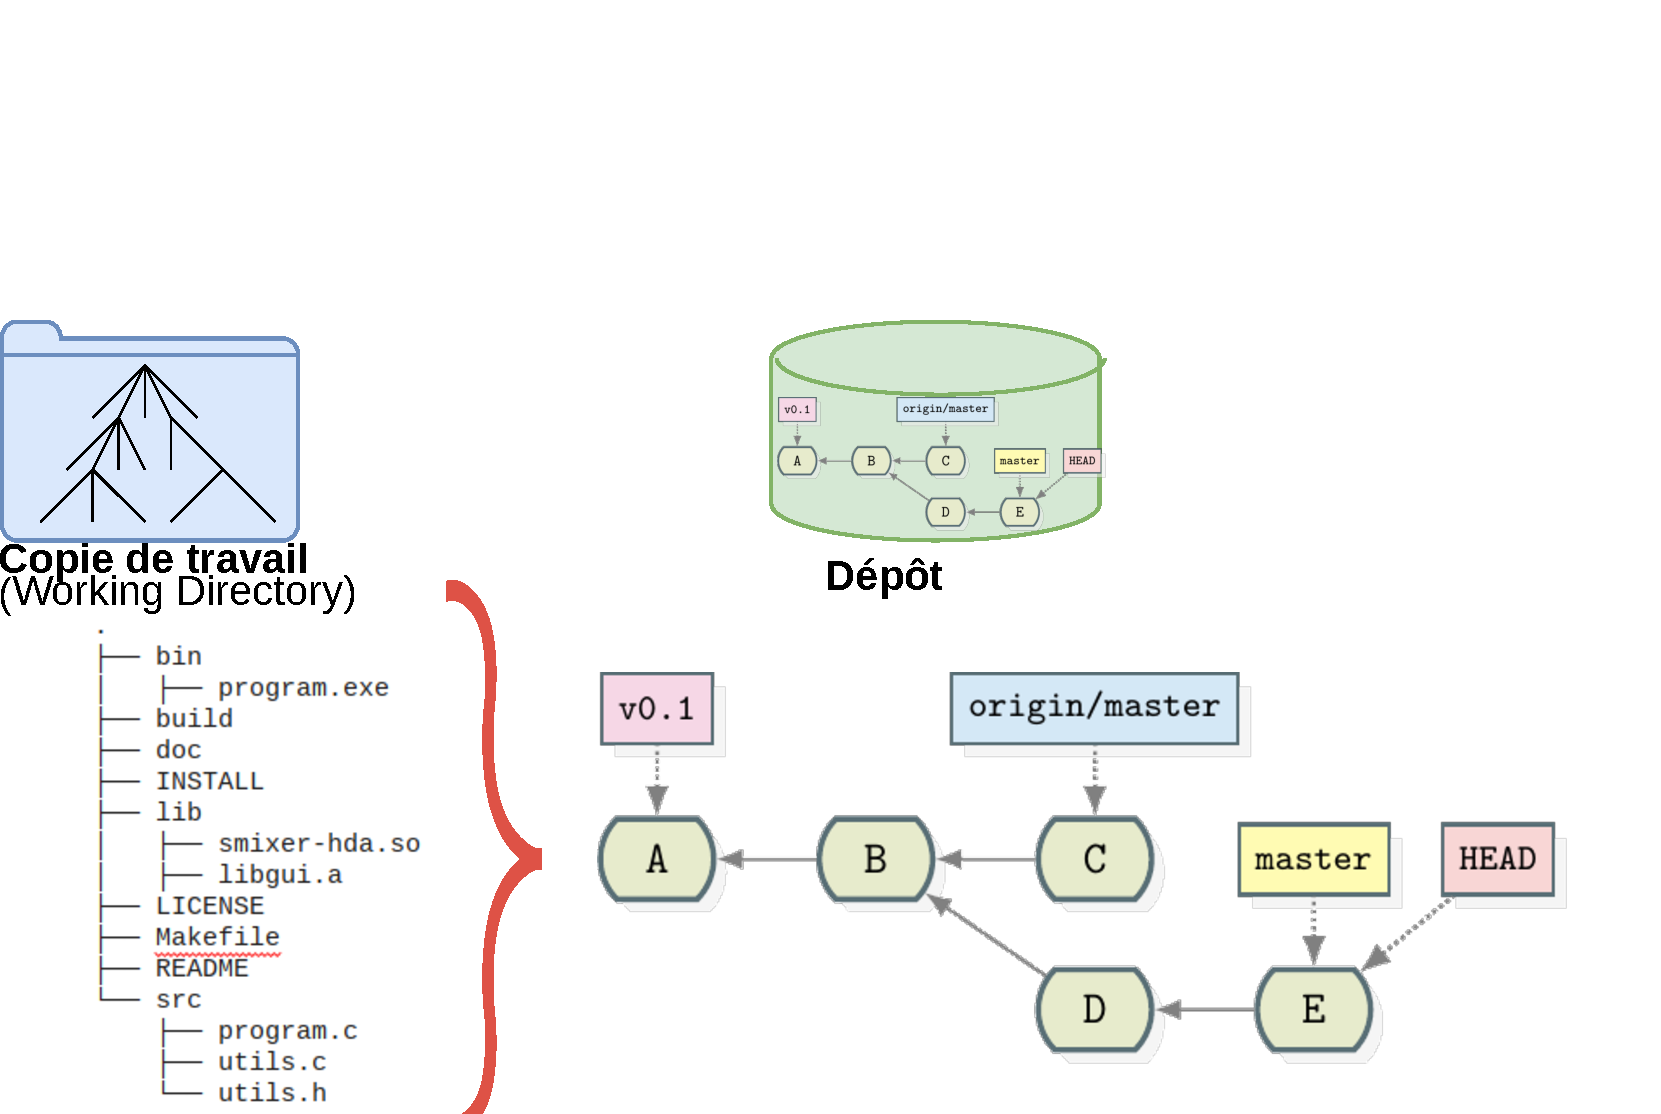
\includegraphics[scale=0.44]{images/workflow2.pdf}}}\stepcounter{numSlide}
			\only<\value{numSlide}>{{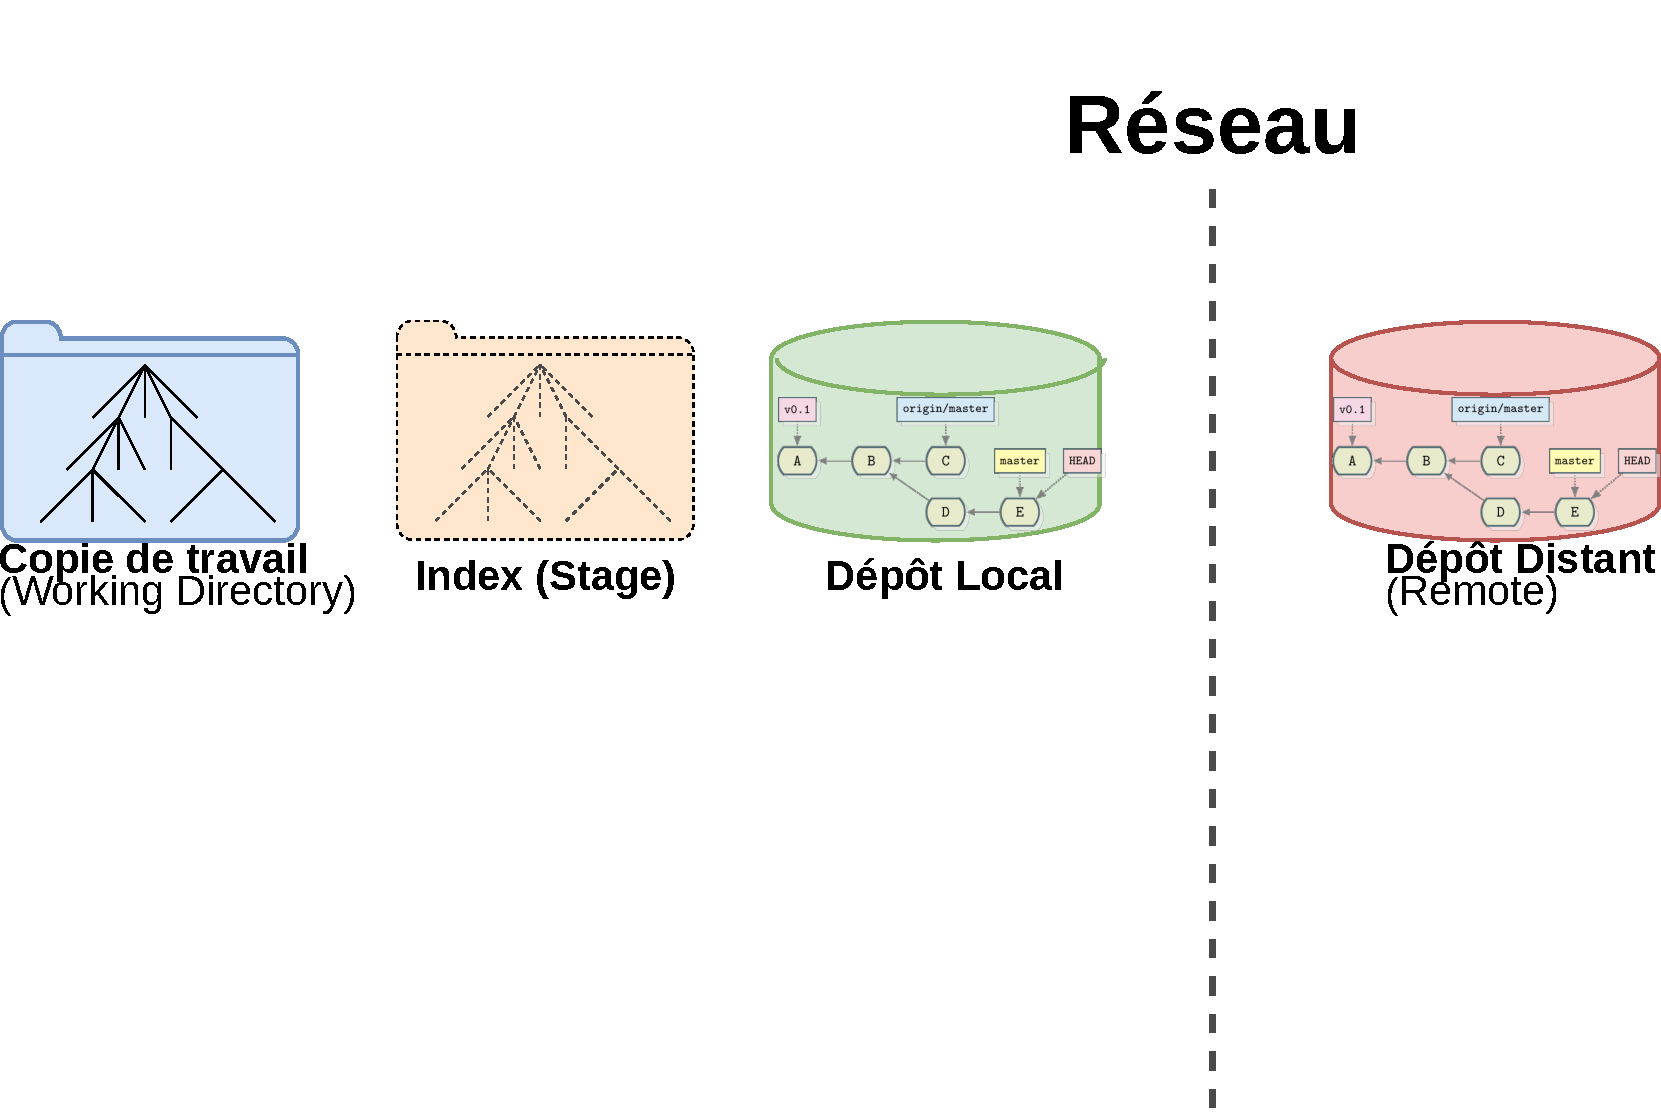
\includegraphics[scale=0.44]{images/workflow3.pdf}}}\stepcounter{numSlide}
		\fi
		\only<\value{numSlide}>{{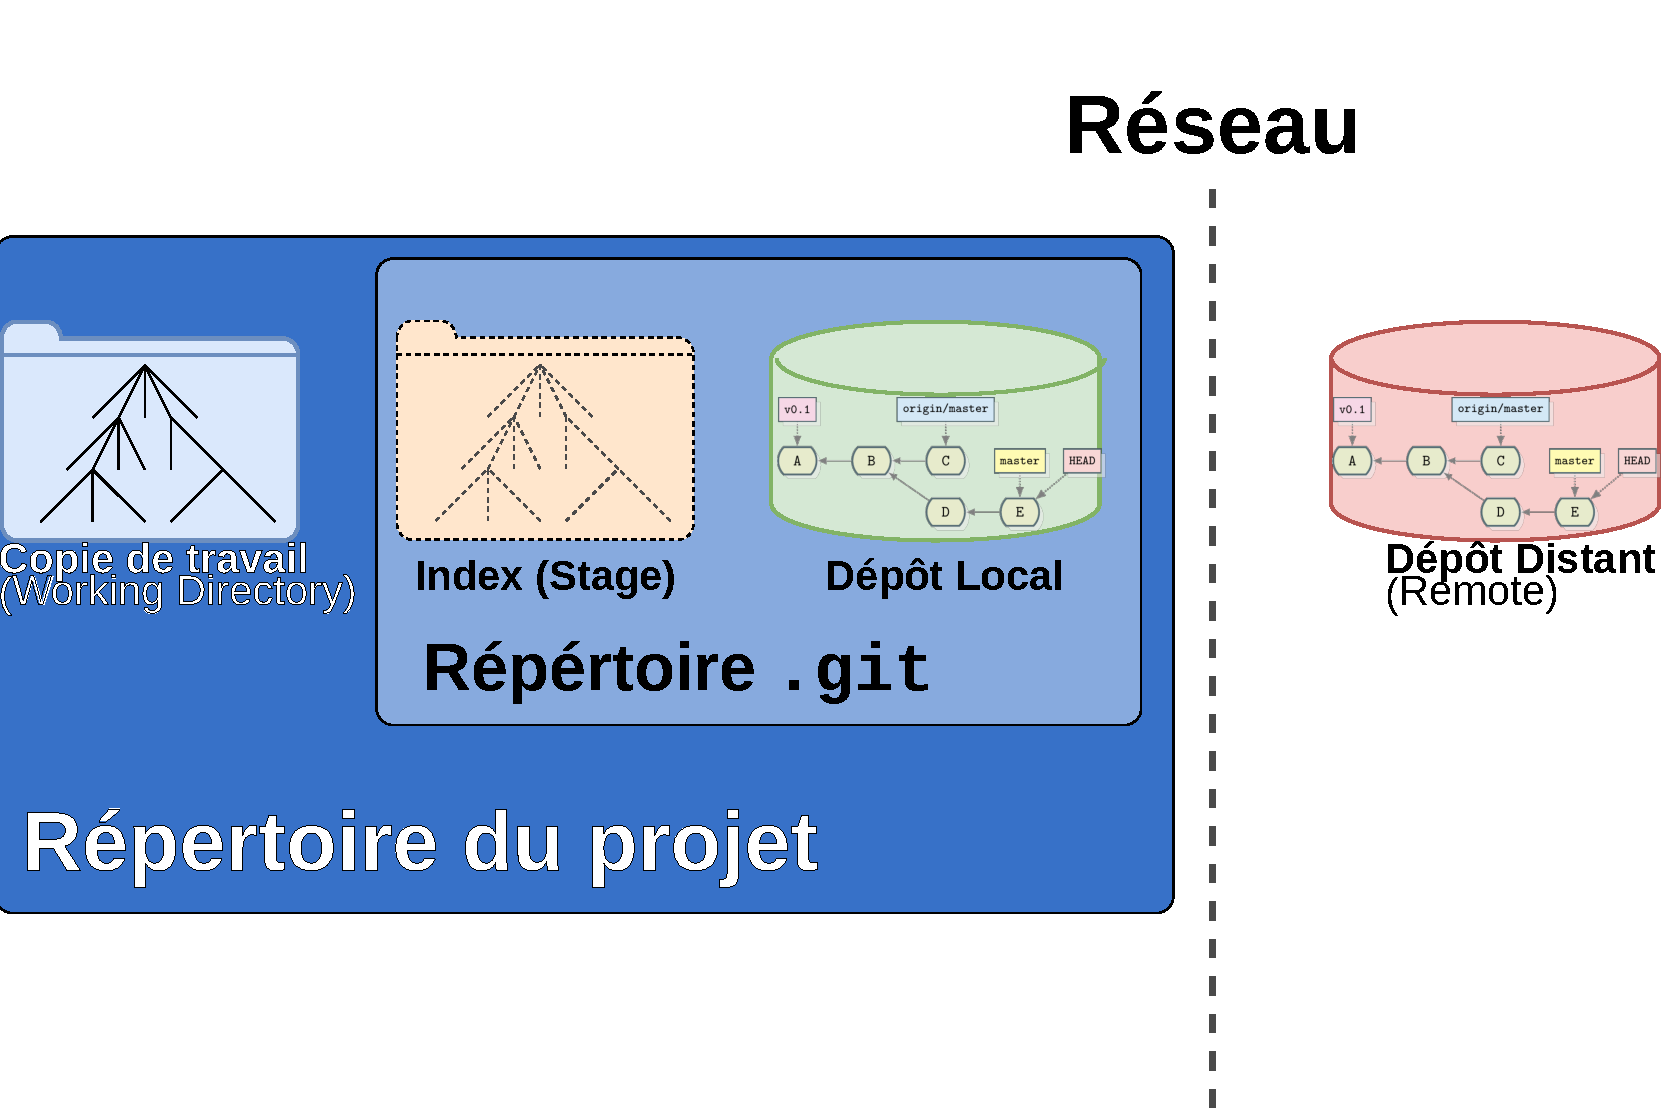
\includegraphics[scale=0.44]{images/workflow4.pdf}}}\stepcounter{numSlide}
		\ifANIMATE
			\only<\value{numSlide}>{{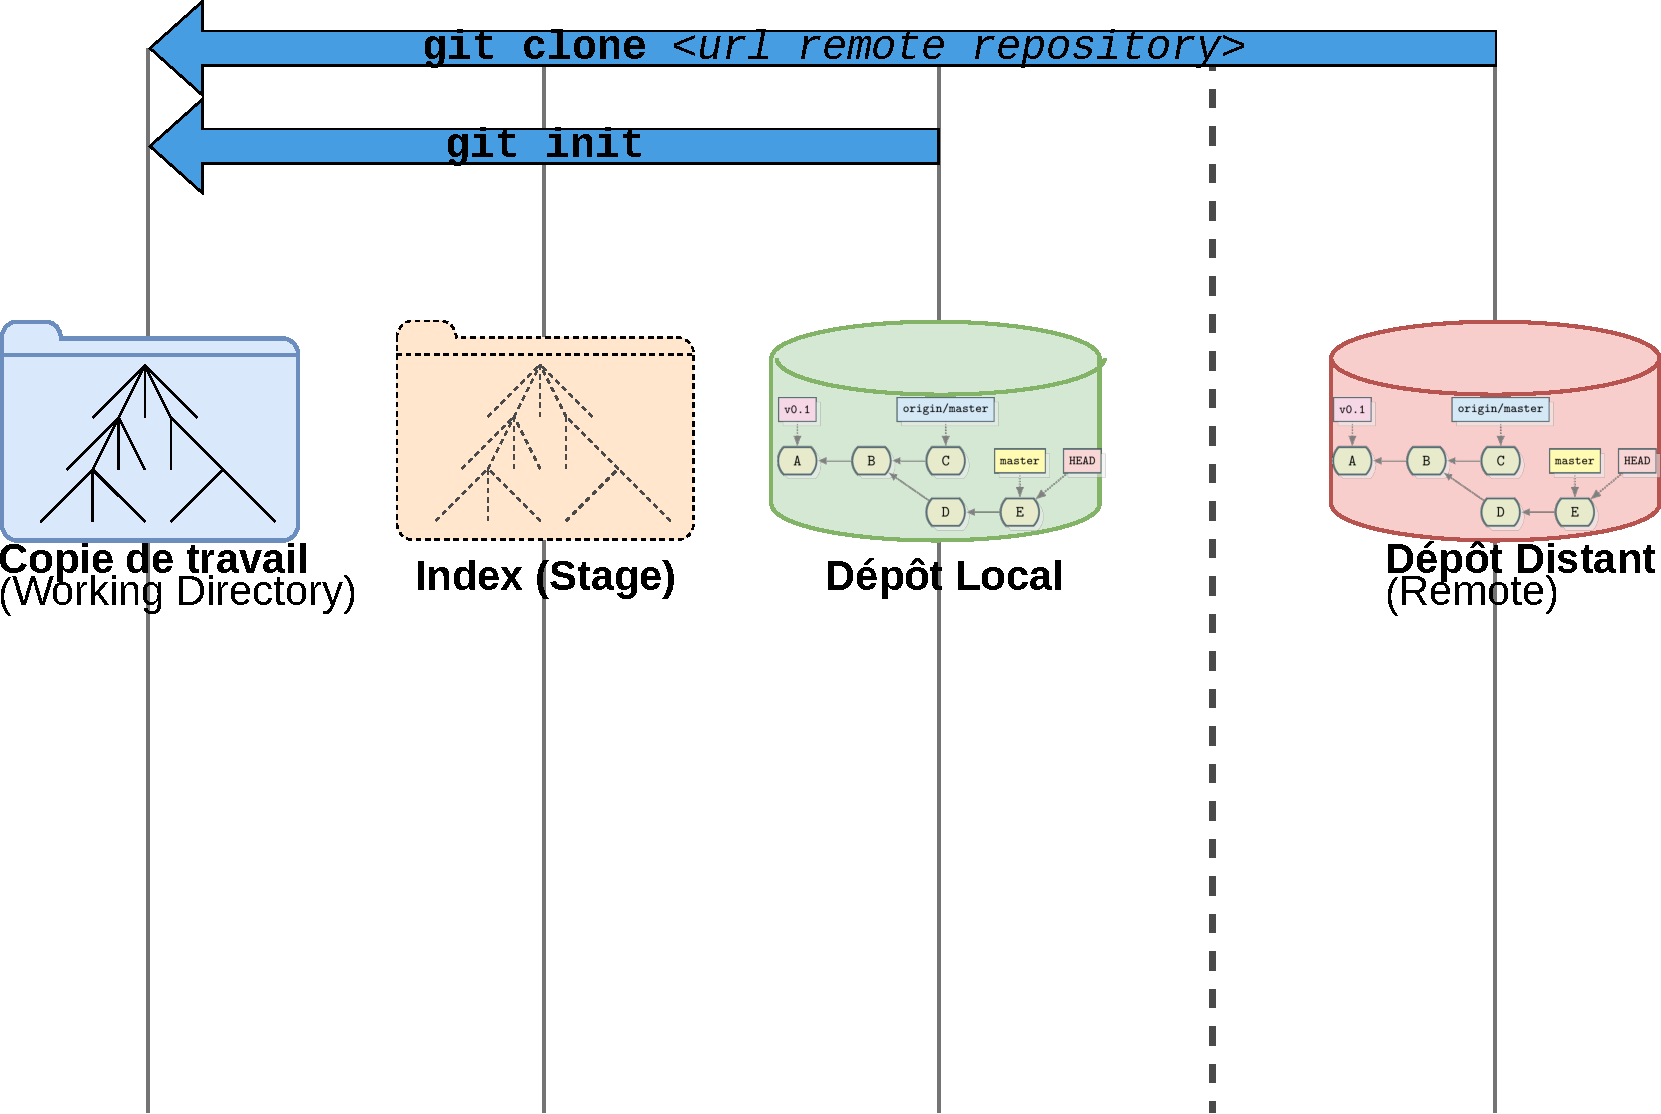
\includegraphics[scale=0.44]{images/workflow5.pdf}}}\stepcounter{numSlide}
			\only<\value{numSlide}>{{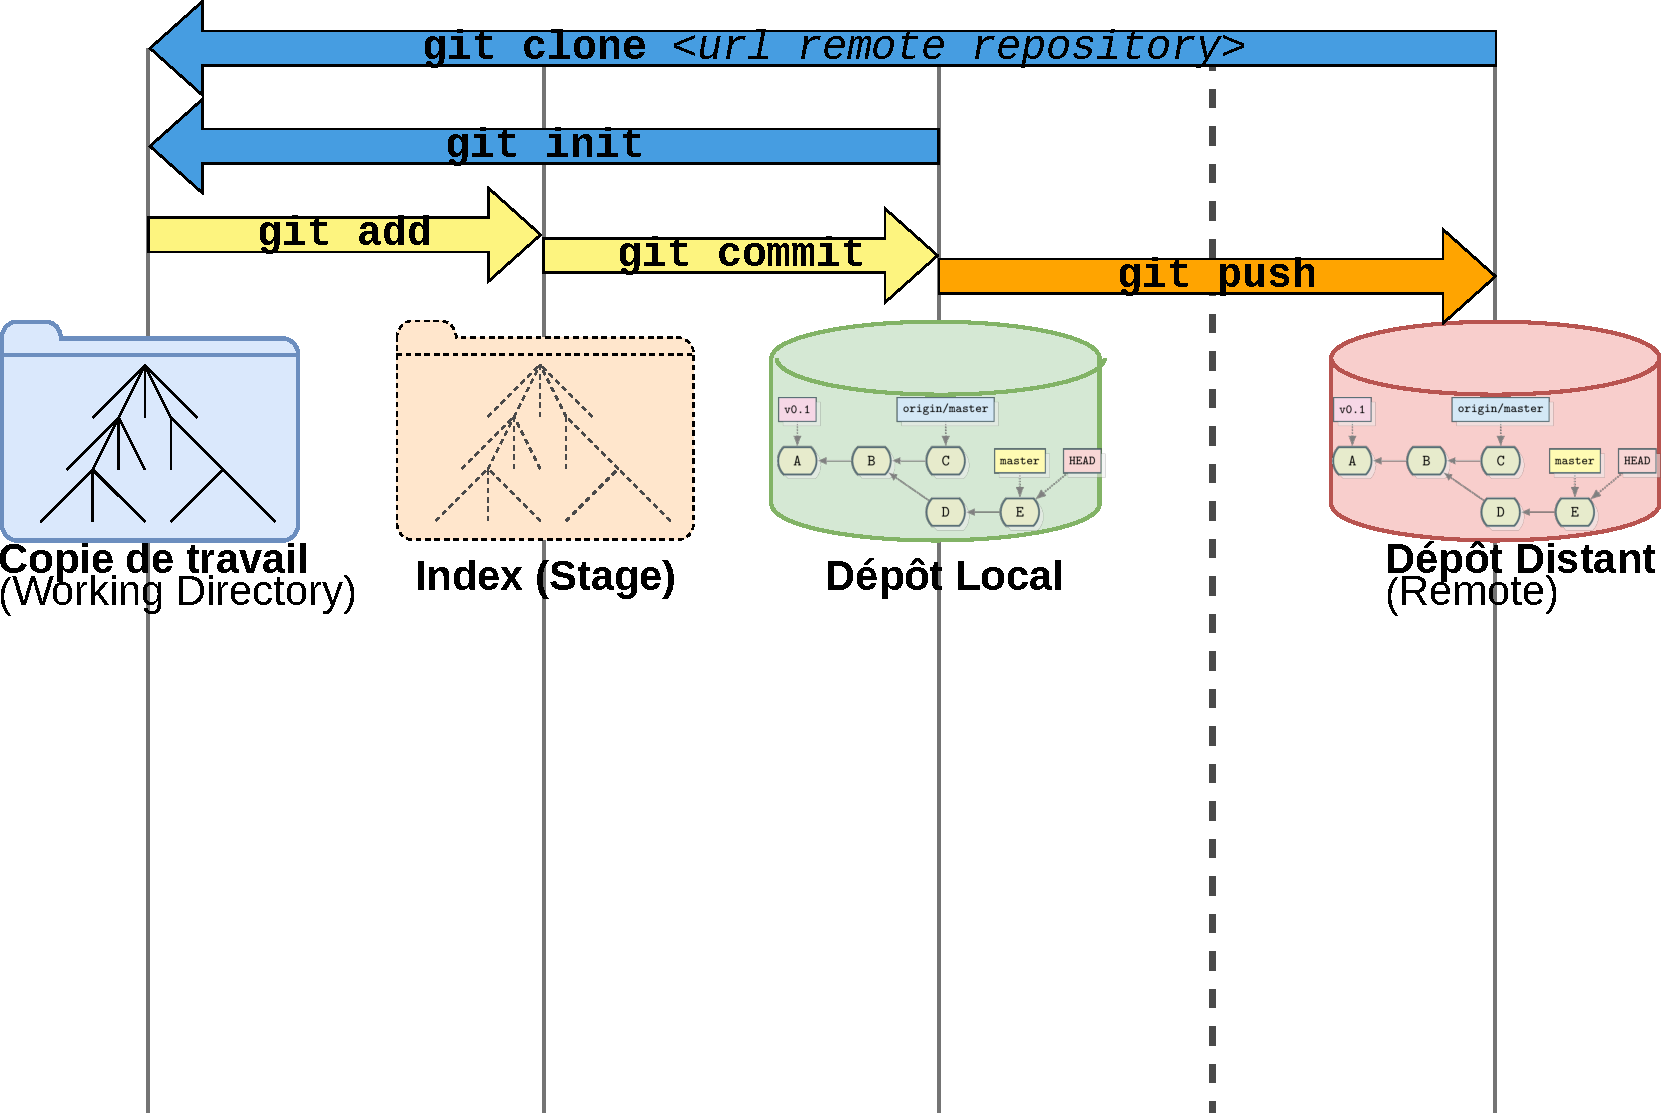
\includegraphics[scale=0.44]{images/workflow6.pdf}}}\stepcounter{numSlide}
			\only<\value{numSlide}>{{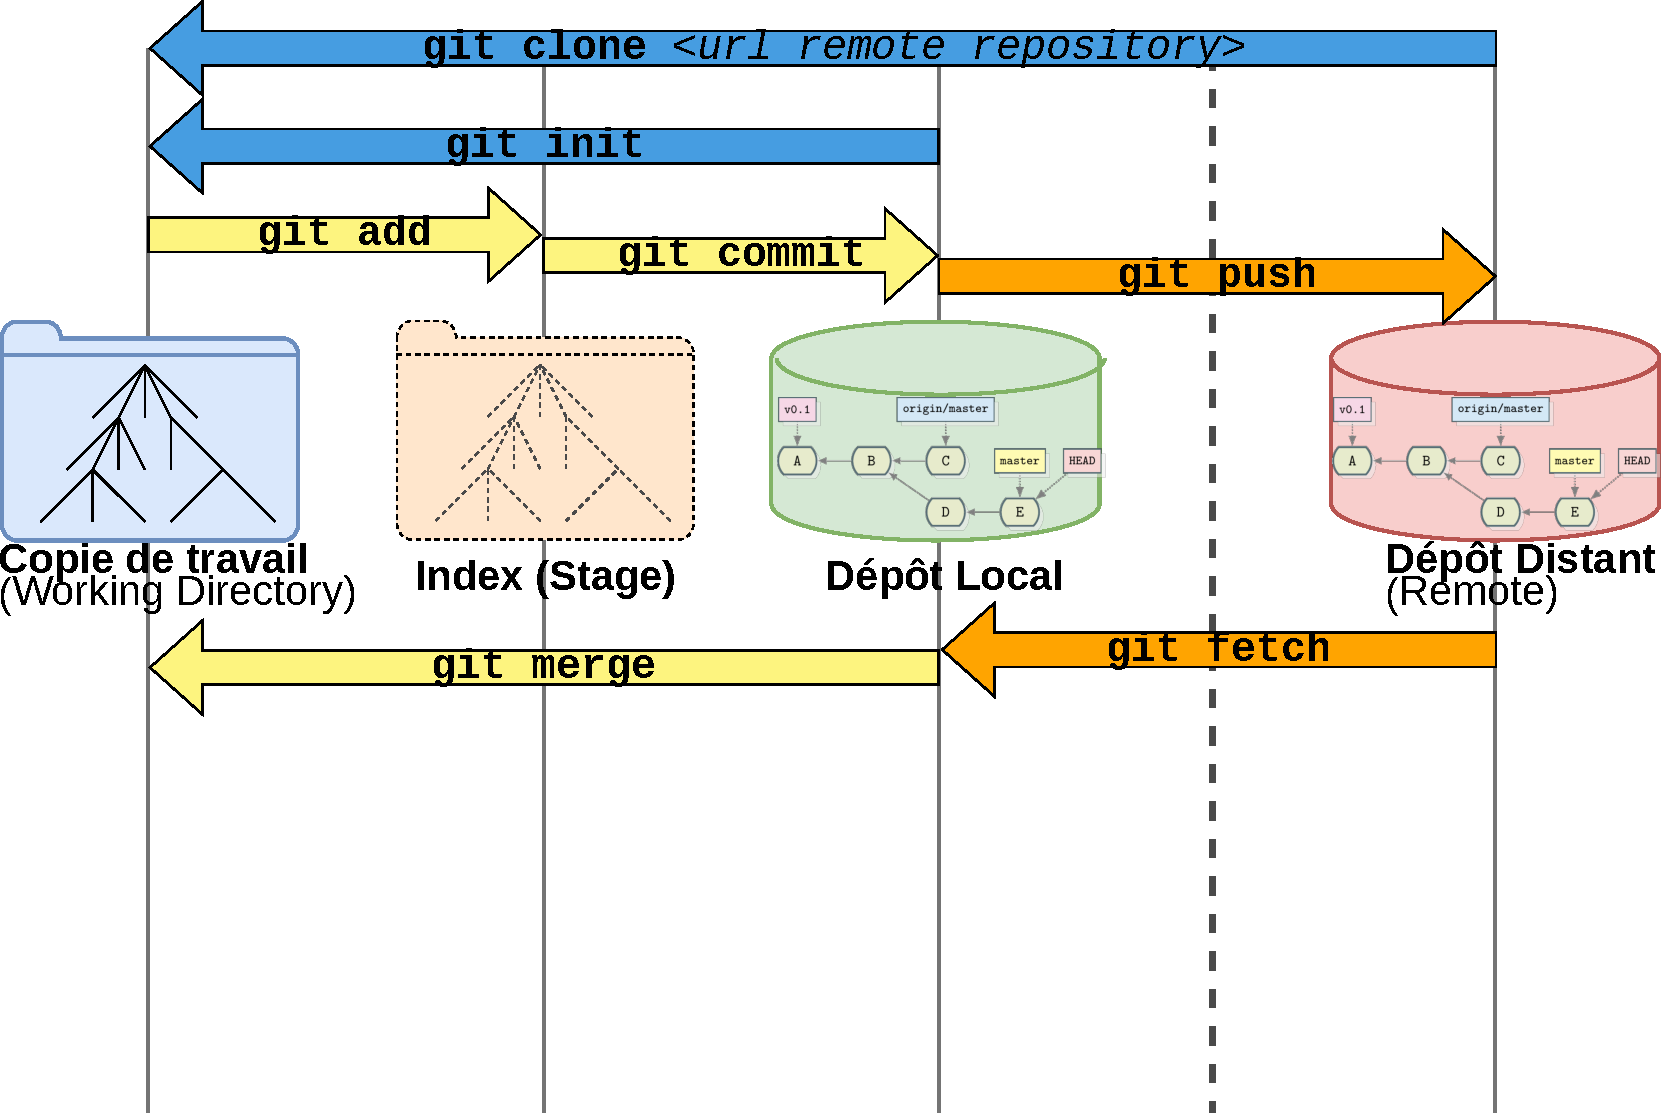
\includegraphics[scale=0.44]{images/workflow7.pdf}}}\stepcounter{numSlide}
			\only<\value{numSlide}>{{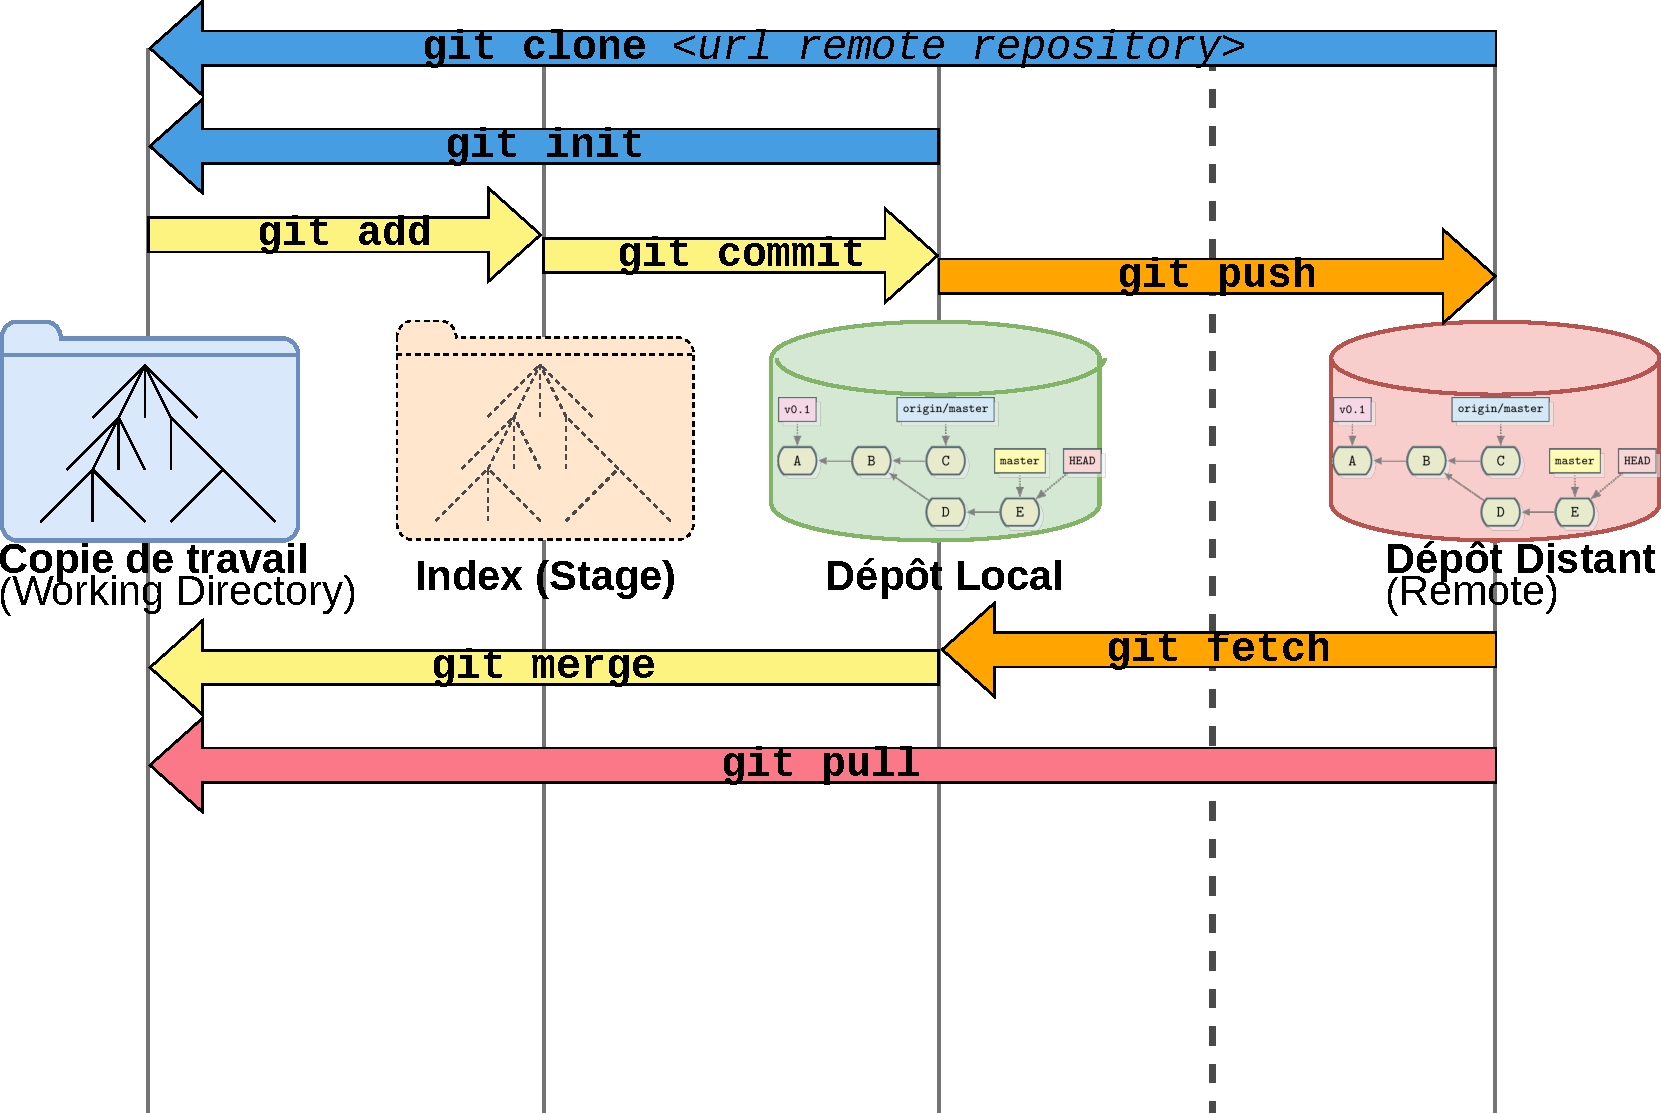
\includegraphics[scale=0.44]{images/workflow8.pdf}}}\stepcounter{numSlide}
			%\only<\value{numSlide}>{{\includegraphics[scale=0.44]{images/workflow9.pdf}}}
			%\stepcounter{numSlide}
			%\only<\value{numSlide}>{{\includegraphics[scale=0.44]{images/workflow10.pdf}}}
			%\stepcounter{numSlide}
		\fi
		\only<\value{numSlide}>{{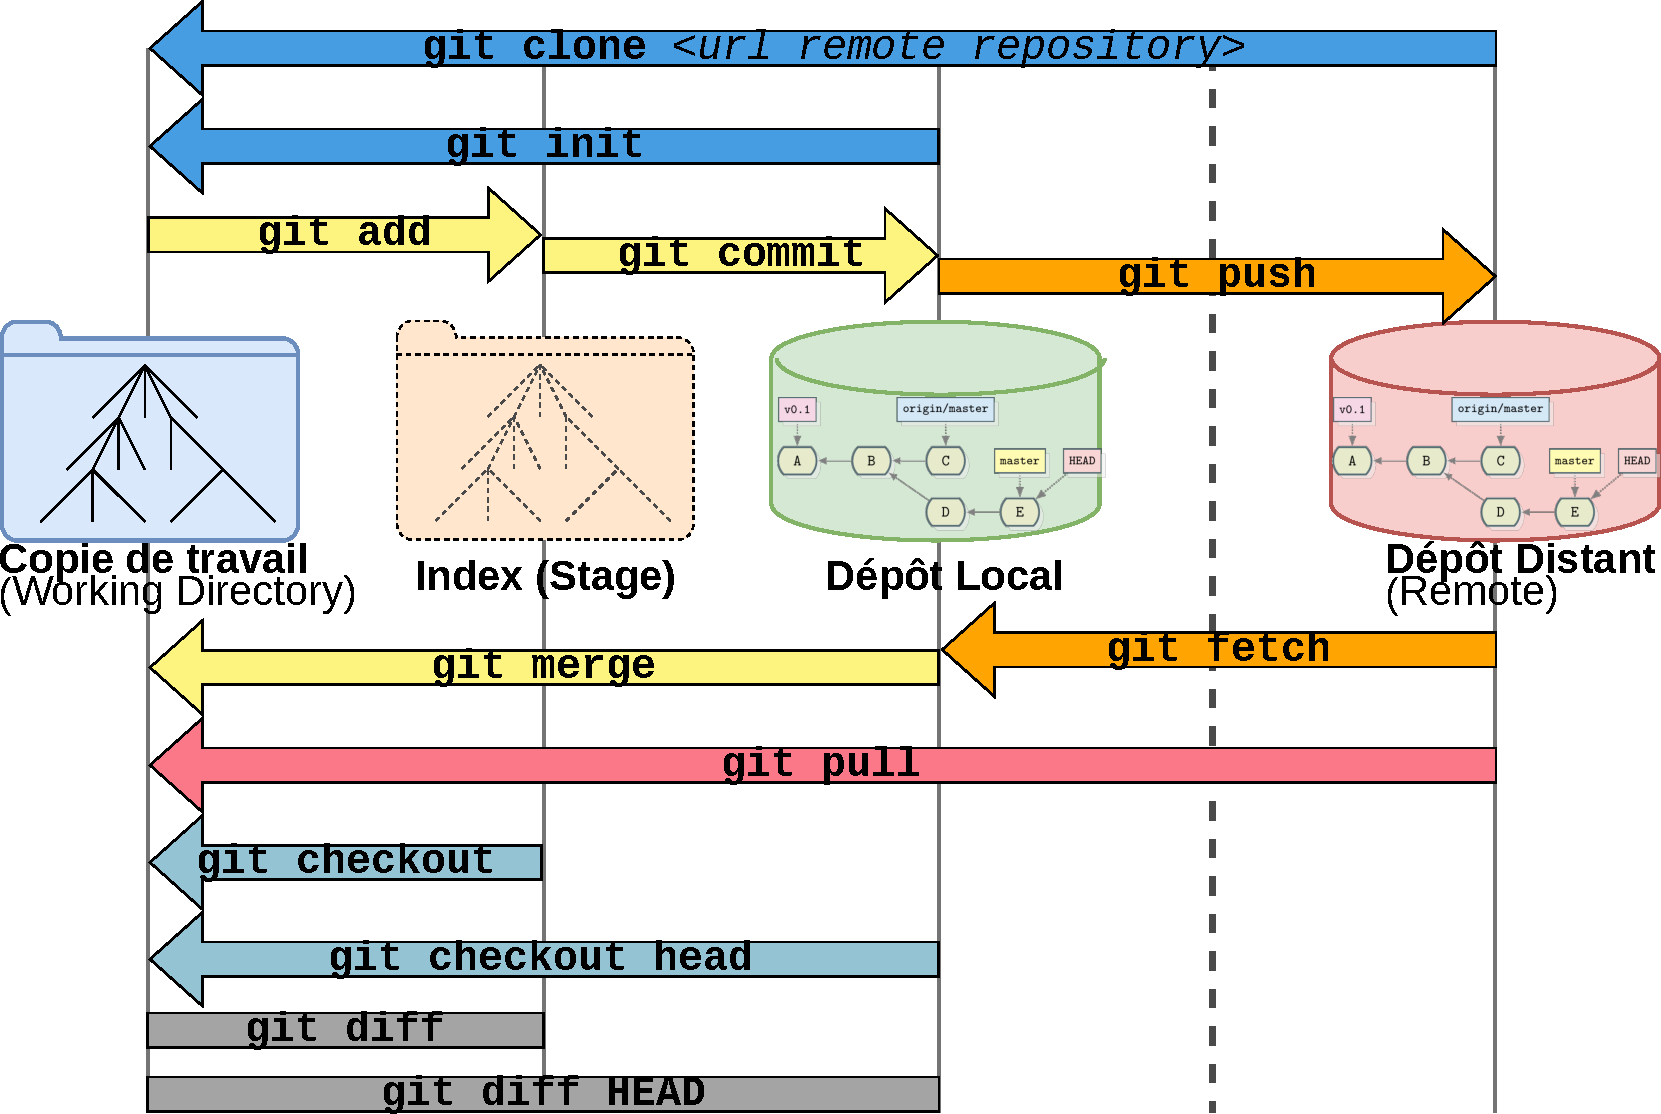
\includegraphics[scale=0.44]{images/workflow_all.pdf}}}
	\end{center}
\end{adjustwidth}
\end{frame}



%%%%%%%%%% Begin Premier Commit
\begin{frame}[fragile]
%\frametitle{The Directed Acyclic \textit{Commit}-Graph in Git}
\frametitle{Le \textit{Graphe Orienté Acyclique} de \texttt{commits}}
%	\vspace{-0.5cm}
 	\begin{figure}
	%\only<2->{
	\onslide<2>{
		\begin{subfigure}[h]{\textwidth}
		%\centering
		\begin{tikzpicture}
		% Commit DAG
		\gitDAG[grow right sep = 2em]{
			27ff4
		};
		% Tag reference
	%	\gittag [v0p1] {v0.1} {above=of A} {A}
		% Remote branch
		% Branch
		\gitbranch
		{master}     % node name and text 
		{above=of 27ff4} % node placement
		{27ff4}          % target
		% HEAD reference
		\gitHEAD
		%	 			{above=of master} % node placement
		{right=of master} % node placement
		{master}          % target
		\end{tikzpicture}
		\end{subfigure}
	}
	\subcaption{\only<1>{Dépôt vide}\only<2->{Premier \textit{commit}}}
	\end{figure}

	\begin{block}{Dans un terminal \ldots}
	\begin{overprint}
	\onslide<1>
	\vspace{-0.3cm}
	\begin{semiTransparentBox}
	\begin{minted}[mathescape=true,escapeinside=||,tabsize=4
	,fontsize=\footnotesize,
	]{c}
	mkdir mon_depot ; cd mon_depot
	git init .
	echo "pomme" |>{}>| fruits.txt
	git add fruits.txt
	git commit -m "Pomme ajouté à la liste de fruits"
	  |$\Rightarrow$| ID = 27ff4
	\end{minted}
	\end{semiTransparentBox}

%	\onslide<1>{
%	\begin{semiTransparentBox}
	\onslide<2>
	\vspace{-0.3cm}
	\begin{solidBox}
	\begin{minted}[mathescape=true,escapeinside=||,tabsize=4
	,fontsize=\footnotesize,
	]{c}
	mkdir mon_depot ; cd mon_depot
	git init .
	echo "pomme" |>{}>| fruits.txt
	git add fruits.txt
	git commit -m "Pomme ajouté à la liste de fruits"
	  |$\Rightarrow$| ID = 27ff4
	\end{minted}
	\end{solidBox}
	\end{overprint}
%	\end{semiTransparentBox}
%	}
	\end{block}

	\onslide<2>{
		\vspace{0.5cm}
		Faire \textbf{\texttt{ git status}} et \textbf{\texttt{ git log}} \underline{après toute commande}!
	}
\end{frame}
%%%%%%%%%% End Premier Commit


\begin{frame}
\frametitle{C'est quoi un commit ?}
	\vspace{-1em}
	\begin{block}{}
	\begin{adjustwidth}{-0.5cm}{-0.5cm}{}
		\begin{center}	
			{\includegraphics[scale=0.6]{images/git_commit.png}}
		\end{center}
	\end{adjustwidth}
	\end{block}

	\vspace{-2em}
	\begin{block}{}
	%    \begin{adjustwidth}{-0.9cm}{}
	\begin{itemize}
		\item Le \texttt{Commit-ID} est une \textit{empreinte} calculé en utilisant la fonction de hachage \texttt{SHA-1} sur
		\begin{itemize}
			\item \textbf{Tout} le contenu du commit + Date + Nom et email du commiteur + Message de log + ID du commit parent + \ldots
		\end{itemize}
	\end{itemize}
	%	\end{adjustwidth}
%	\begin{itemize}
%	\item 
	Propriété : \textbf{Unicité} quasi-universelle de l'\texttt{ID}
%	\begin{itemize}
%		\item Unicité universelle statistique de l'ID
%	\end{itemize}
%\end{itemize}
%	\end{adjustwidth}
\end{block}
\end{frame}


%\newcounter{numSlide}
%%%%%%%%%%% ANIMATION Commit 2
\begin{frame}[fragile]
%\frametitle{The DAG in Git : Commit 2}
\frametitle{Le Graphe : Commit 2}

\setcounter{numSlide}{1}

\only<\value{numSlide}>{
	\begin{figure}
		\begin{subfigure}[h]{\textwidth}
			%\centering
			\begin{tikzpicture}
			% Commit DAG
			\gitDAG[grow right sep = 2em]{
				27ff4
			};
			\gitbranch
			{master}     % node name and text 
			{above=of 27ff4} % node placement
			{27ff4}          % target
			% HEAD reference
			\gitHEAD
			%	 			{above=of master} % node placement
			{right=of master} % node placement
			{master}          % target
			\end{tikzpicture}
			\subcaption{État avant deuxième \texttt{commit}}
		\end{subfigure}
	\end{figure}
}
\stepcounter{numSlide}
\only<\value{numSlide}>{
	\begin{figure}
		\begin{subfigure}[h]{\textwidth}
			%\centering
			\begin{tikzpicture}
			% Commit DAG
			\gitDAG[grow right sep = 2em]{
				27ff4 -- 31490
			};
			\gitbranch
			{master}     % node name and text 
			{above=of 31490} % node placement
			{31490}          % target
			% HEAD reference
			\gitHEAD
			%	 			{above=of master} % node placement
			{right=of master} % node placement
			{master}          % target
			\end{tikzpicture}
			\subcaption{Deuxième \textit{commit}}
		\end{subfigure}
	\end{figure}
}

%\vspace{-0.5cm}
%\vspace{0.4cm} \begin{center} \noindent\makebox[\linewidth]{\line(2,0){500}} \end{center} \vspace{-0.4cm} 
\begin{block}{Dans un terminal \ldots}<1->
%	\vspace{-0.2cm}		
	\begin{minted}[mathescape=true,escapeinside=||,tabsize=4
	,fontsize=\footnotesize,
	]{c}
	echo banane |>{}>| fruits.txt
	git add fruits.txt
	git commit -m "Ajouté banane à fruits.txt"
	  |$\Rightarrow$| ID = 31490
	\end{minted}
\end{block}

\only<1>{\begin{tikzpicture}[remember picture,overlay]\node[xshift=1.3cm,yshift=3.4cm] at (current page.south west) {$\hookrightarrow$};\end{tikzpicture}}
\only<2>{\begin{tikzpicture}[remember picture,overlay]\node[xshift=1.3cm,yshift=1.8cm] at (current page.south west) {$\hookrightarrow$};\end{tikzpicture}}

\end{frame}
%%%%%%%%%%% End ANIMATION Commit 2


%%%%%%%%%%% ANIMATION Commit 3
\begin{frame}[fragile]
%\frametitle{The DAG in Git : Commit 3}
\frametitle{Le Graphe : Commit 3}
	\begin{figure}
		\begin{subfigure}[h]{\textwidth}
			%\centering
			\begin{tikzpicture}
			% Commit DAG
			\gitDAG[grow right sep = 2em]{
				27ff4 -- 31490 -- ab5d1
			};
			% Tag reference
			%	\gittag [v0p1] {v0.1} {above=of A} {A}
			% Remote branch
			% Branch
			\gitbranch
			{master}     % node name and text 
			{above=of ab5d1} % node placement
			{ab5d1}          % target
			% HEAD reference
			\gitHEAD
			%	 			{above=of master} % node placement
			{right=of master} % node placement
			{master}          % target
			\end{tikzpicture}
			\subcaption{Troisième \textit{commit}}
		\end{subfigure}
	\end{figure}

%\vspace{-0.5cm}
\begin{block}{Dans un terminal \ldots}
%	\vspace{-0.2cm}
%	\vspace{0.4cm} \begin{center} \noindent\makebox[\linewidth]{\line(2,0){500}} \end{center} \vspace{-0.4cm} 		
	\begin{minted}[mathescape=true,escapeinside=||,tabsize=4,fontsize=\footnotesize
	%,linenos,
	]{c}
	echo orange |>{}>| fruits.txt
	git add fruits.txt
	git commit -m "Ajouté orange à fruits.txt"
	  |$\Rightarrow$| ID = ab5d1
	\end{minted}
\end{block}
\end{frame}
%%%%%%%%%%% End ANIMATION Commit 3


%%%%%%%%%%% ANIMATION Branch 1
\begin{frame}[fragile]
\frametitle{Le Graphe : Branche \texttt{legumes}}

\setcounter{numSlide}{0}

\ifANIMATE
	\stepcounter{numSlide}
	\only<\value{numSlide}>{
		\begin{figure}
		\begin{subfigure}[h]{\textwidth}
			%\centering
			\begin{tikzpicture}
			% Commit DAG
			\gitDAG[grow right sep = 2em]{
				27ff4 -- 31490 -- ab5d1
			};
			% Tag reference
			%	\gittag [v0p1] {v0.1} {above=of A} {A}
			% Remote branch
			% Branch
			\gitbranch
			{master}     % node name and text 
			{above=of ab5d1} % node placement
			{ab5d1}          % target
			% HEAD reference
			\gitHEAD
			%	 			{above=of master} % node placement
			{right=of master} % node placement
			{master}          % target
			\end{tikzpicture}
			\subcaption{Avant branche}
		\end{subfigure}
		\end{figure}
	}
\fi

\stepcounter{numSlide}
\only<\value{numSlide}%
\ifANIMATE
	-\the\numexpr\value{numSlide}+1
\fi%
>{
		\begin{figure}
		\begin{subfigure}[h]{\textwidth}
			%\centering
			\begin{tikzpicture}
			% Commit DAG
			\gitDAG[grow right sep = 2em]{
				27ff4 -- 31490 -- ab5d1
			};
			% Tag reference
			%	\gittag [v0p1] {v0.1} {above=of A} {A}
			% Remote branch
			% Branch
			\gitbranch
			{master}     % node name and text 
			{above=of ab5d1} % node placement
			{ab5d1}          % target
			\gitbranch {legumes} {right=of master} {ab5d1}
			\gitHEAD
			%	 			{above=of master} % node placement
			{right=of legumes} % node placement
			{legumes}          % target
	
			\end{tikzpicture}
			\subcaption{Après branche}
%\ifANIMATE
			\vspace{-0.7em}
			\only<\the\numexpr\value{numSlide}>{
				$\Rightarrow$ une nouvelle \textit{étiquette} (\texttt{legumes}) apparait, elle pointe vers le commit courant (\texttt{ab5d1}), et la commande \texttt{checkout} fait pointer \texttt{HEAD} sur \texttt{legumes}
				%elle pointe vers le même \texttt{commit} que \texttt{HEAD}
%				\vspace{-1.65em}
%				\vspace{-4.1em}%Perfect for animation
				\vspace{-3.4em}
%				\ifANIMATE
%					\vspace{-2em}
%				\fi
			}
%\fi
\ifANIMATE
			\stepcounter{numSlide}
\fi
		\end{subfigure}
	\end{figure}
}

\stepcounter{numSlide}
\only<\value{numSlide}
%%%%%%%%%%%%%%%%%%%% BUG HERE
%%%%%%%%%%%%%%%%%%%%
%%%%%%%%%%%%%%%%%%%% HAD TO PUT 2 HERE OR ELSE SLIDE WOULDN'T SHOW TWICE
\ifANIMATE
	-\the\numexpr\value{numSlide}+2
\fi
>{
\ifANIMATE
	\stepcounter{numSlide}
	\stepcounter{numSlide}
\fi
	\begin{figure}
		\begin{subfigure}[h]{\textwidth}
			%\centering
			\begin{tikzpicture}
			% Commit DAG
			\gitDAG[grow right sep = 2em]{
				27ff4 -- 31490 -- ab5d1 -- ffd5c
			};
			% Tag reference
%			\gittag [v0p1] {v0.1} {above=of 27ff4} {27ff4}
%			 Remote branch
%			 Branch
			\gitbranch
			{master}     % node name and text 
			{above=of ab5d1} % node placement
			{ab5d1}          % target
			\gitbranch {legumes} {above=of ffd5c} {ffd5c}
			% HEAD reference
			\gitHEAD
 			{right=of legumes} % node placement
%			{right=of legumes} % node placement
%			{ffd5c}          % target
			{legumes}          % target
			
			\end{tikzpicture}
			\subcaption{Après un premier commit dans la branche \texttt{legumes}}
		\end{subfigure}
	\end{figure}
}

\ifANIMATE
	\stepcounter{numSlide}
	\stepcounter{numSlide}
\fi

%\only<\value{numSlide}
%		\ifANIMATE
%				-\the\numexpr\value{numSlide}+1
%		\fi
%>{
%\ifANIMATE
	\stepcounter{numSlide}
%\fi

\only<\value{numSlide}>{
	\begin{figure}
		\begin{subfigure}[h]{\textwidth}
			%\centering
			\begin{tikzpicture}
			% Commit DAG
			\gitDAG[grow right sep = 2em]{
				27ff4 -- 31490 -- ab5d1 -- ffd5c -- 8a928
			};
			% Tag reference
			%	\gittag [v0p1] {v0.1} {above=of A} {A}
			% Remote branch
			% Branch
			\gitbranch
			{master}     % node name and text 
			{above=of ab5d1} % node placement
			{ab5d1}          % target
%			% HEAD reference
%			\gitHEAD
%			{below=of 8a928} % node placement
%			%			{right=of legumes} % node placement
%			{8a928}          % target
			\gitbranch {legumes} {above=of 8a928} {8a928}
			% HEAD reference
			\gitHEAD
			{right=of legumes} % node placement
			%			{right=of legumes} % node placement
			{legumes}          % target

			\end{tikzpicture}
			\subcaption{Après un deuxième commit dans la branche \texttt{legumes}}
		\end{subfigure}
	\end{figure}
}

\ifANIMATE
	\only<1>{\begin{tikzpicture}[remember picture,overlay]\node[xshift=1.3cm,yshift=3.5cm] at (current page.south west) {$\hookrightarrow$};\end{tikzpicture}}
	\only<2-3>{\begin{tikzpicture}[remember picture,overlay]\node[xshift=1.3cm,yshift=2.85cm] at (current page.south west) {$\hookrightarrow$};\end{tikzpicture}}
	\only<4-5>{\begin{tikzpicture}[remember picture,overlay]\node[xshift=1.3cm,yshift=1.4cm] at (current page.south west) {$\hookrightarrow$};\end{tikzpicture}}
	\only<6->{\begin{tikzpicture}[remember picture,overlay]\node[xshift=1.3cm,yshift=0.2cm] at (current page.south west) {$\hookrightarrow$};\end{tikzpicture}}
\fi

	\vspace{0.4cm} \begin{center} \noindent\makebox[\linewidth]{\line(2,0){500}} \end{center} \vspace{-0.4cm}
	\begin{minted}[mathescape=true,escapeinside=||,tabsize=4,fontsize=\footnotesize,]{c}
	git branch legumes ; git checkout legumes
	\end{minted}
	
	\pause
	\PAUSE
	\begin{minted}[mathescape=true,escapeinside=||,tabsize=4,fontsize=\footnotesize,]{c}
	echo aubergine |>{}>| legumes.txt ; git add legumes.txt
	git commit -m "Ajout aubergine à legumes"
	  |$\Rightarrow$| ID = ffd5c
	\end{minted}
	\pause
	\PAUSE
	\begin{minted}[mathescape=true,escapeinside=||,tabsize=4,fontsize=\footnotesize,]{c}
	echo courgette |>{}>| legumes.txt ; git add legumes.txt
	git commit -m "Ajout courgette à legumes"
	  |$\Rightarrow$| ID = 8a928
	\end{minted}
\end{frame}
%%%%%%%%%%% End ANIMATION Branch 1



%%%%%%%%%%% ANIMATION Branch 2
\begin{frame}[fragile]
\frametitle{Le Graphe : Branche \texttt{master}}

\setcounter{numSlide}{0}

\ifANIMATE
	\stepcounter{numSlide}
	\only<\value{numSlide}>{
%	\only<1>{
	\begin{figure}
		\begin{subfigure}[h]{\textwidth}
			%\centering
			\begin{tikzpicture}
			% Commit DAG
			\gitDAG[grow right sep = 2em]{
				27ff4 -- 31490 -- ab5d1 -- ffd5c -- 8a928
			};
			% Tag reference
			%	\gittag [v0p1] {v0.1} {above=of A} {A}
			% Remote branch
			% Branch
			\gitbranch
			{master}     % node name and text 
			{above=of ab5d1} % node placement
			{ab5d1}          % target
			% HEAD reference
			\gitHEAD
			{right=of master} % node placement
			%			{right=of legumes} % node placement
			{master}          % target
			\gitbranch {legumes} {above=of 8a928} {8a928}
			
			\end{tikzpicture}
			\subcaption{Travaillons sur \texttt{master}}
		\end{subfigure}
	\end{figure}
	}
\fi

\stepcounter{numSlide}
\only<\value{numSlide}>{ %
%\ifANIMATE %instead of repeating this slide, I turned it into another one below.
%	-\the\numexpr\value{numSlide}+1
%\fi%
%>{
%\only<2-3>{
	\begin{figure}
		\begin{subfigure}[h]{\textwidth}
			%\centering
			\begin{tikzpicture}
			% Commit DAG
			\gitDAG[grow right sep = 2em]{
				27ff4 -- 31490 -- ab5d1 -- ffd5c -- 8a928
			};
			% Tag reference
			%	\gittag [v0p1] {v0.1} {above=of A} {A}
			% Remote branch
			% Branch
			\gitbranch
			{master}     % node name and text 
			{above=of ab5d1} % node placement
			{ab5d1}          % target
			% HEAD reference
			\gitHEAD
			{right=of master} % node placement
			%			{right=of legumes} % node placement
			{master}          % target
			\gitbranch {legumes} {above=of 8a928} {8a928}
			
			\end{tikzpicture}
			\subcaption{Travaillons sur \texttt{master}}
			%\only<2>{
			\only<\the\numexpr\value{numSlide}>{$\Rightarrow$ \texttt{legumes.txt} n'existe plus dans la Copie de Travail (\textit{Working Directory})}
%			\vspace{0.33em}
			\vspace{-2.93em}
		\end{subfigure}
	\end{figure}
}

%\stepcounter{numSlide}
\stepcounter{numSlide}

%\ifANIMATE %Et si on commite ?
\only<\value{numSlide}>{
	\begin{figure}
		\begin{subfigure}[h]{\textwidth}
			%\centering
			\begin{tikzpicture}
			% Commit DAG
			\gitDAG[grow right sep = 2em]{
				27ff4 -- 31490 -- ab5d1 -- ffd5c -- 8a928
			};
			% Tag reference
			%	\gittag [v0p1] {v0.1} {above=of A} {A}
			% Remote branch
			% Branch
			\gitbranch
			{master}     % node name and text 
			{above=of ab5d1} % node placement
			{ab5d1}          % target
			% HEAD reference
			\gitHEAD
			{right=of master} % node placement
			%			{right=of legumes} % node placement
			{master}          % target
			\gitbranch {legumes} {above=of 8a928} {8a928}
			
			\end{tikzpicture}
			\subcaption{Et si on commite sur \texttt{master} ?}
%			\vspace{2.2em}
		\end{subfigure}
	\end{figure}
}
	\stepcounter{numSlide}
%\fi

\only<\value{numSlide}
%\ifANIMATE
%	-\the\numexpr\value{numSlide}+1
%\fi
>{
%\only<4>{
	\begin{figure}
		\begin{subfigure}[h]{\textwidth}
			%\centering
			\begin{tikzpicture}
			% Commit DAG
			\gitDAG[grow right sep = 2em]{
				27ff4 -- 31490 -- ab5d1 -- {ffd5c -- 8a928, 21721}
			};
			% Tag reference
			%	\gittag [v0p1] {v0.1} {above=of A} {A}
			% Remote branch
			% Branch
			\gitbranch
			{master}     % node name and text 
			{below=of 21721} % node placement
			{21721}          % target
			% HEAD reference
			\gitHEAD
			{right=of master} % node placement
			%			{right=of legumes} % node placement
			{master}          % target
			\gitbranch {legumes} {above=of 8a928} {8a928}
			
			\end{tikzpicture}
			\subcaption{Après un nouveau \textit{commit} sur \texttt{master}}
			\vspace{-4em}
		\end{subfigure}
	\end{figure}
}

\vspace{0.4cm}
\begin{center} \noindent\makebox[\linewidth]{\line(2,0){500}} \end{center} \vspace{-0.4cm}
\begin{minted}[mathescape=true,escapeinside=||,tabsize=4,fontsize=\footnotesize,]{c}
	git checkout master
\end{minted}

\ifANIMATE
	\only<1-3>{\begin{tikzpicture}[remember picture,overlay]\node[xshift=1.3cm,yshift=2.7cm] at (current page.south west) {$\hookrightarrow$};\end{tikzpicture}}
%	\only<2>{\begin{tikzpicture}[remember picture,overlay]\node[xshift=1.3cm,yshift=2.7cm] at (current page.south west) {$\hookrightarrow$};\end{tikzpicture}}
\fi
\pause
%\pause
\PAUSE
\begin{minted}[mathescape=true,escapeinside=||,tabsize=4,fontsize=\footnotesize,]{c}
	echo poire |>{}>| fruits.txt ; git add fruits.txt
	git commit -m "Ajouté poire à fruits.txt"
		|$\Rightarrow$| ID = 21721
\end{minted}

\ifANIMATE
%	\only<3>{\begin{tikzpicture}[remember picture,overlay]\node[xshift=1.3cm,yshift=2.7cm] at (current page.south west) {$\hookrightarrow$};\end{tikzpicture}}
	\only<4->{\begin{tikzpicture}[remember picture,overlay]\node[xshift=1.3cm,yshift=0.6cm] at (current page.south west) {$\hookrightarrow$};\end{tikzpicture}}
\fi
\end{frame}
%%%%%%%%%%% End ANIMATION Branch 2


%%%%%%%%%%% ANIMATION Merge 1
\begin{frame}[fragile]
\frametitle{Le Graphe : Merge \texttt{master}\Rightarrow\texttt{legumes}}
\only<1>{
	\begin{figure}
		\begin{subfigure}[h]{\textwidth}
			%\centering
			\begin{tikzpicture}
			% Commit DAG
			\gitDAG[grow right sep = 1.5em]{
				27ff4 -- 31490 -- ab5d1 -- {ffd5c -- 8a928, 21721}
			};
			% Tag reference
			%	\gittag [v0p1] {v0.1} {above=of A} {A}
			% Remote branch
			% Branch
			\gitbranch
			{master}     % node name and text 
			{below=of 21721} % node placement
			{21721}          % target
			\gitbranch {legumes} {above=of 8a928} {8a928}
			\gitHEAD
			{right=of legumes} % node placement
			{legumes}          % target

			
			\end{tikzpicture}
			\subcaption{Allons sur \texttt{légumes}, regardons les différences avec \texttt{diff}}
			%\only<2>{$\Longrightarrow$ \texttt{legumes.txt} n'existe plus dans \textit{Working Directory})}
		\end{subfigure}
	\end{figure}
}

\only<2>{
	\begin{figure}
		\begin{subfigure}[h]{\textwidth}
			%\centering
			\begin{tikzpicture}
			% Commit DAG
			\gitDAG[grow right sep = 1.5em]{
				27ff4 -- 31490 -- ab5d1 -- {ffd5c -- 8a928, 21721} -- 760cf
			};
			% Tag reference
			%	\gittag [v0p1] {v0.1} {above=of A} {A}
			% Remote branch
			% Branch
			\gitbranch
			{master}     % node name and text 
			{below=of 21721} % node placement
			{21721}          % target
			\gitbranch {legumes} {above=of 760cf} {760cf}
			\gitHEAD
			{left=of legumes} % node placement
			%			{right=of legumes} % node placement
			{legumes}          % target
			
			\end{tikzpicture}
			\subcaption{Merger \texttt{master} dans \texttt{légumes} : produit un \underline{nouveau commit}}
			%\only<2>{$\Longrightarrow$ \texttt{legumes.txt} n'existe plus dans \textit{Working Directory})}
		\end{subfigure}
	\end{figure}
}

\vspace{-0.5cm}
%\only<2-3>{
%\begin{block}{Sur le terminal \ldots}
%\pause[2]
%\vspace{-0.2cm}
\vspace{0.4cm} \begin{center} \noindent\makebox[\linewidth]{\line(2,0){500}} \end{center} \vspace{-0.4cm}
\begin{minted}[mathescape=true,escapeinside=||,tabsize=4,fontsize=\footnotesize,]{c}
	git checkout legumes
\end{minted}

%\only<1>{\begin{tikzpicture}[remember picture,overlay]\node[xshift=1.3cm,yshift=1.7cm] at (current page.south west) {$\hookrightarrow$};\end{tikzpicture}}
%\pause

\begin{minted}[mathescape=true,escapeinside=||,tabsize=4,fontsize=\footnotesize,]{c}
	git diff master
\end{minted}
\begin{minted}[mathescape=true,escapeinside=||,tabsize=4,fontsize=\footnotesize,]{c}
	git merge master
\end{minted}

\only<1>{\begin{tikzpicture}[remember picture,overlay]\node[xshift=1.3cm,yshift=1.3cm] at (current page.south west) {$\hookrightarrow$};\end{tikzpicture}}

\pause
%\begin{minted}[mathescape=true,escapeinside=||,tabsize=4,fontsize=\footnotesize,]{c}
%	git merge master
%\end{minted}
\only<2>{\begin{tikzpicture}[remember picture,overlay]\node[xshift=1.3cm,yshift=0.7cm] at (current page.south west) {$\hookrightarrow$};\end{tikzpicture}}
\end{frame}
%%%%%%%%%%% End ANIMATION Merge 1

\begin{frame}[fragile]
\frametitle{Merge : Vue dans la console}
%\begin{block}{Représentation par pointeurs}%Parcours postfixé ou \texttt{GRD}}
\begin{adjustwidth}{-1cm}{-0.8cm}{}
	\begin{center}
		{\includegraphics[scale=0.3]{images/git_log_merge.png}}
		\begin{minted}[mathescape=true,escapeinside=||,tabsize=4,fontsize=\footnotesize,]{c}
			git log |-{}-|all |-{}-|graph |-{}-|oneline |-{}-|date=short
		\end{minted}
	\end{center}
\end{adjustwidth}
%\end{block}
\end{frame}



%%%%%%%%%%% ANIMATION Merge 2
\begin{frame}[fragile]
\frametitle{Le Graphe : Merge \texttt{legumes}\Rightarrow \texttt{master}}
\only<1>{
	\begin{figure}
		\begin{subfigure}[h]{\textwidth}
			%\centering
			\begin{tikzpicture}
			% Commit DAG
			\gitDAG[grow right sep = 1.5em]{
				27ff4 -- 31490 -- ab5d1 -- {ffd5c -- 8a928, 21721} -- 760cf
			};
			% Tag reference
			%	\gittag [v0p1] {v0.1} {above=of A} {A}
			% Remote branch
			% Branch
			\gitbranch
			{master}     % node name and text 
			{below=of 21721} % node placement
			{21721}          % target
			% HEAD reference
			\gitHEAD
			{right=of master} % node placement
			%			{right=of legumes} % node placement
			{master}          % target
			\gitbranch {legumes} {above=of 760cf} {760cf}
			
			\end{tikzpicture}
			\subcaption{Allons sur \texttt{master}}
			%\only<2>{$\Longrightarrow$ \texttt{legumes.txt} n'existe plus dans \textit{Working Directory})}
		\end{subfigure}
	\end{figure}
}

\only<2>{
	\begin{figure}
		\begin{subfigure}[h]{\textwidth}
			%\centering
			\begin{tikzpicture}
			% Commit DAG
			\gitDAG[grow right sep = 1.5em]{
				27ff4 -- 31490 -- ab5d1 -- {ffd5c -- 8a928, 21721} -- 760cf
			};
			% Tag reference
			%	\gittag [v0p1] {v0.1} {above=of A} {A}
			% Remote branch
			% Branch
			\gitbranch
			{master}     % node name and text 
			{below=of 760cf} % node placement
			{760cf}          % target
			% HEAD reference
			\gitbranch {legumes} {above=of 760cf} {760cf}
			\gitHEAD
			{left=of master} % node placement
			%			{right=of legumes} % node placement
			{master}          % target			
			\end{tikzpicture}
			\subcaption{Merger \texttt{légumes} dans \texttt{master} : \underline{pas de nouveau commit}}
			%\only<2>{$\Longrightarrow$ \texttt{legumes.txt} n'existe plus dans \textit{Working Directory})}
		\end{subfigure}
	\end{figure}
}

\only<3>{
	\begin{figure}
		\begin{subfigure}[h]{\textwidth}
			%\centering
			\begin{tikzpicture}
			% Commit DAG
			\gitDAG[grow right sep = 1.5em]{
				27ff4 -- 31490 -- ab5d1 -- {ffd5c -- 8a928, 21721} -- 760cf
			};
			% Tag reference
			%	\gittag [v0p1] {v0.1} {above=of A} {A}
			% Remote branch
			% Branch
			\gitbranch
			{master}     % node name and text 
			{above=of 760cf} % node placement
			{760cf}          % target
			% HEAD reference
			\gitHEAD
			{left=of master} % node placement
			%			{right=of legumes} % node placement
			{master}          % target
%			\gitbranch {legumes} {above=of 760cf} {760cf}
			
			\end{tikzpicture}
			\subcaption{Effacer la branche \texttt{légumes}}
			%\only<2>{$\Longrightarrow$ \texttt{legumes.txt} n'existe plus dans \textit{Working Directory})}
		\end{subfigure}
	\end{figure}
}
\vspace{0.4cm} \begin{center} \noindent\makebox[\linewidth]{\line(2,0){500}} \end{center} \vspace{-0.4cm}

\only<1>{\vspace{0.5em}}
\begin{minted}[mathescape=true,escapeinside=||,tabsize=4,fontsize=\footnotesize,]{c}
	git checkout master
\end{minted}
\begin{minted}[mathescape=true,escapeinside=||,tabsize=4,fontsize=\footnotesize,]{c}
	git diff legumes
	git merge legumes
\end{minted}
\begin{minted}[mathescape=true,escapeinside=||,tabsize=4,fontsize=\footnotesize,]{c}
	git branch -d legumes
\end{minted}

\only<1>{\begin{tikzpicture}[remember picture,overlay]\node[xshift=1.3cm,yshift=1.95cm] at (current page.south west) {$\hookrightarrow$};\end{tikzpicture}}

\pause[2]
\only<2>{\begin{tikzpicture}[remember picture,overlay]\node[xshift=1.3cm,yshift=1.3cm] at (current page.south west) {$\hookrightarrow$};\end{tikzpicture}}
\pause
\only<3->{\begin{tikzpicture}[remember picture,overlay]\node[xshift=1.3cm,yshift=0.7cm] at (current page.south west) {$\hookrightarrow$};\end{tikzpicture}}
\end{frame}
%%%%%%%%%%% End ANIMATION Merge 2



%\begin{frame}{TODO: Origin}
%
%All previous parts show how the graph is constructed locally.
%
%TODO: EXPLAIN HOW TO PUSH/PULL BETWEEN DIFFERENT REPOSITORIES.
%MERGING, KEEPING UP TO DATE, ORIGIN/MASTER TAG.
%
%This should describe how the "distributed" part of Git Works.
%
%%\begin{minted}[mathescape=true,escapeinside=||,tabsize=4
%%	%,fontsize=\footnotesize,
%%	]{c}
%%	echo "pommes" |>{}>| fruits.txt
%%\end{minted}
%\end{frame}


\begin{frame}{Partager : dépôts distants}
\begin{adjustwidth}{-0.75cm}{0cm}{}
\vspace{-1em}
	\begin{center}
		\only<1>{{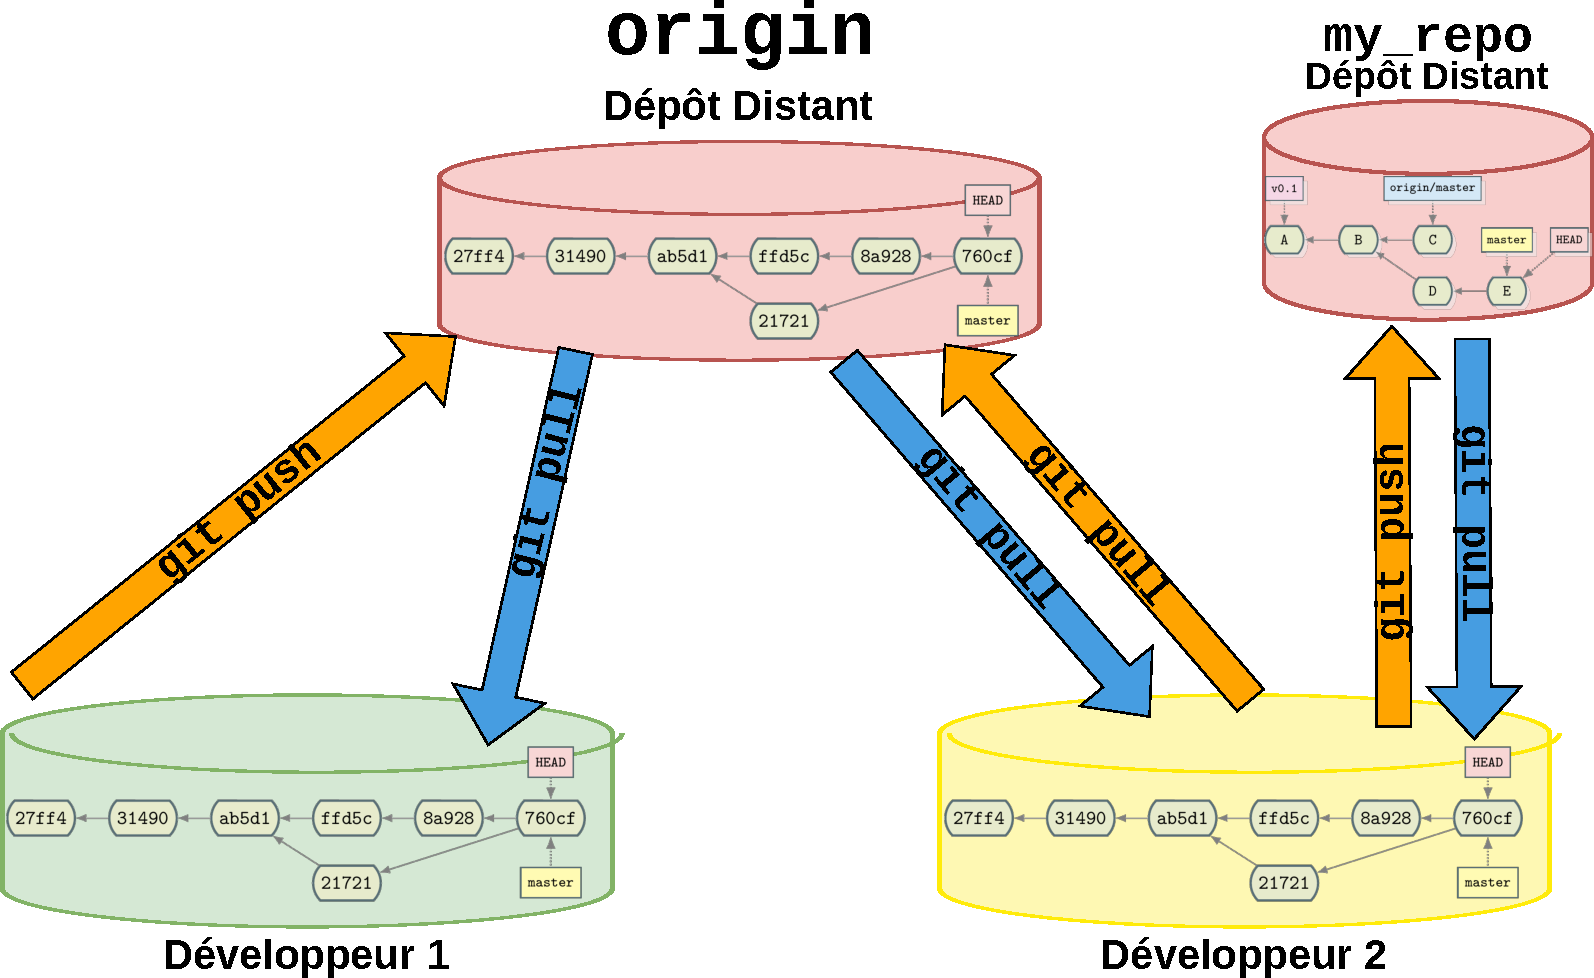
\includegraphics[scale=0.44]{images/remote_origin.pdf}}}
	\end{center}
\end{adjustwidth}
\end{frame}


%%%%%%%%%%%%%%%%%%%%%%%%%%%%%%%%%%%%%%%%%%%%%%%%%%%%%%%%%%%%%%%%%%%%%%%%%%%%%%%%%%%%%%%%%%%%%%
\begin{frame}[fragile]
%\frametitle{Git distribué : Gestion Centralisée}
\frametitle{Dépôt Centralisée : \textit{initialisation}}
\begin{adjustwidth}{-2em}{0cm}{}
\color{darkgreen}%\rule{\linewidth}{4pt}
\noindent
Premier commit \\ \small(dépôt central doit être créé et vide)
\color{black}
\end{adjustwidth}
\begin{adjustwidth}{-1em}{0cm}{}
\begin{minted}[mathescape=true,escapeinside=**,tabsize=4,fontsize=\footnotesize,linenos,breaklines,
numbersep=5pt,
]{bash}
git init .
git add .
git commit -m "first commit"

git remote add origin git@github.com:rudametw/Learning-Git-Test-Repo.git
git push -u origin master
\end{minted}
\end{adjustwidth}

\begin{adjustwidth}{-0cm}{0cm}{}
	\begin{columns}[T] % align columns
		\begin{column}{.6\textwidth}
		\end{column}%
		%\hfill%
%		\color{darkgreen}\rule{\linewidth}{4pt}
		\begin{column}{.3\textwidth}
%			\color{blue}\rule{\linewidth}{4pt}
%			Workflow \textit{(édité à la main)}
			\color{black}
			\vspace{-11em}
			\begin{adjustwidth}{-0cm}{-3cm}{}
				\begin{figure}
					\hfill
					\includegraphics[scale=0.22]{images/centralized_workflow.png}
				\end{figure}
			\end{adjustwidth}
		\end{column}%
	\end{columns}
	\vspace{-1em}
	\PAUSE
	\color{darkgray}\rule{\linewidth}{2pt}
%	\begin{columns}[T] % align columns
%	\begin{column}{.5\textwidth}
	
	\begin{adjustwidth}{-0.5cm}{-3cm}{}
		\color{darkgreen}%\rule{\linewidth}{4pt}
		Chaque développeur \texttt{clone} une seule fois
		\color{black}
		\begin{minted}[mathescape=true,escapeinside=**,tabsize=4,fontsize=\footnotesize,linenos,
		numbersep=5pt,
		]{bash}
git clone https://github.com/rudametw/Learning-Git-Test-Repo.git
cd Learning-Git-Test-Repo/
git remote -v #permet de vérifier les addresses
		\end{minted}
		\end{adjustwidth}
	\end{adjustwidth}
\end{frame}

%%%%%%%%%%%%%%%%%%%%%%%%%%%%%%%%%%%%%%%%%%%%%%%%%%%%%%%%%%%%%%%%%%%%%%%%%%%%%%%%%%%%%%%%%%%%%%
%continue previous slide, broken into two
%%%%%%%%%%%%%%%%%%%%%%%%%%%%%%%%%%%%%%%%%%%%%%%%%%%%%%%%%%%%%%%%%%%%%%%%%%%%%%%%%%%%%%%%%%%%%%

\begin{frame}[fragile]
%\frametitle{Git distribué : Gestion Centralisée}
\frametitle{Dépôt Centralisée :\textit{ méthode de travail}}
\begin{adjustwidth}{-1em}{0cm}{}
\vspace{-2.3em}
\color{darkgreen}%\rule{\linewidth}{4pt}
Chacun travaille sur une branche \texttt{fonctX}. Une fois la fonctionnalité fini, on merge \texttt{foncX} dans \texttt{master}.\\
\color{black}
\vspace{-1em}
\begin{minted}[mathescape=true,escapeinside=**,tabsize=4,fontsize=\footnotesize,breaklines,
numbersep=5pt,
]{c}
git pull ; git status //update & check work
git branch fonctionalitéX
git checkout fonctionalitéX
\end{minted}

\textit{\texttt{while (je travaille = vrai) $\{$}}
\begin{minted}[mathescape=true,escapeinside=**,tabsize=4,fontsize=\footnotesize,breaklines,numbersep=5pt,]{c}
	git status ; git diff ;
	git add <fichiers>
	git commit -m "message}
\end{minted}
\textit{\texttt{$\}$}}
\begin{minted}[mathescape=true,escapeinside=**,tabsize=4,fontsize=\footnotesize,breaklines,
numbersep=5pt,
]{c}
git pull *-{}-*all
git merge master
//gérér conflits s'il y en a
\end{minted}
\begin{minted}[mathescape=true,escapeinside=**,tabsize=4,fontsize=\footnotesize,breaklines,
numbersep=5pt,
]{c}
//tester que tout marche
git checkout master
git merge fonctionalitéX
git pull ; git push
\end{minted}
\end{adjustwidth}

\vspace{-12em}

\begin{adjustwidth}{-0cm}{-1cm}{}
	\begin{figure}
		\hfill
		\includegraphics[scale=0.22]{images/centralized_workflow.png}
	\end{figure}
\end{adjustwidth}


\end{frame}
%%%%%%%%%%%%%%%%%%%%%%%%%%%%%%%%%%%%%%%%%%%%%%%%%%%%%%%%%%%%%%%%%%%%%%%%%%%%%%%%%%%%%%%%%%%%%%

\begin{frame}
\frametitle{Résolution de conflits}
\begin{block}{Des conflits vont se produire \ldots}
\end{block}
\begin{block}{\ldots comment faire pour les résoudre ?}
\end{block}
\end{frame}

%%%%%%%%%%%%%%%%%%%%%%%%%%%%%%%%%%%%%%%%%%%%%%%%%%%%%%%%%%%%%%%%%%%%%%%%%%%%%%%%%%%%%%%%%%%%%%

%%%%%%%%%%%%%%% CREATION BRANCHE CONFLICTUELLE
\begin{frame}[fragile]
\frametitle{Provoquer un conflit dans \texttt{fruits.txt}}
\vspace{-0.2em}
\begin{adjustwidth}{-0.6cm}{-0.6cm}{}
\begin{columns}[T] % align columns
	\begin{column}{.55\textwidth}
%		\vspace{0.5em}
		\color{darkgreen}
%		{\rule{\linewidth}{3pt}}
		Branche \texttt{ananas}
%		\vspace{+0.4em}
		\color{black}
		\begin{minted}[mathescape=true,escapeinside=||,tabsize=4,fontsize=\footnotesize,breaklines]{bash}
git checkout master
git branch ananas
git checkout ananas
awk 'NR==3\{print "ananas"\}1' fruits.txt > fruits.txt
git add fruits.txt
git commit -m "+ananas"
		\end{minted}
	\end{column}%
	\hfill%
	\begin{column}{.52\textwidth}
		\vspace{-0.2em}
		\color{blue}%\rule{\linewidth}{4pt}
%		+ \texttt{kaki} et - \texttt{orange}
		Branche \texttt{kaki}
		\color{black}
		\vspace{-0.3em}
\begin{minted}[tabsize=4,fontsize=\footnotesize,linenos,breaklines, numbersep=15pt,]{bash}
git checkout master
git branch kaki
git checkout kaki
awk 'NR==3\{print kaki\}1' fruits.txt | grep -v orange > fruits.txt
git add fruits.txt
git commit -m "+kaki -orange"
\end{minted}
\end{column}%
\end{columns}
\end{adjustwidth}

\color{gray}\rule{\linewidth}{3pt}
\color{black}
\vspace{-0.82em}

\PAUSE


%\begin{adjustwidth}{-0.6cm}{-0.6cm}{}
\begin{columns}[T] % align columns
	\begin{column}{.45\textwidth}
%		\vspace{0.5em}
		\color{darkgreen}
%		{\rule{\linewidth}{3pt}}
		Branche \texttt{ananas}
		\texttt{fruits.txt :}
%		\vspace{+0.4em}
		\color{black}
		\begin{minted}[tabsize=4,fontsize=\footnotesize,linenos,breaklines]{bash}
pomme
banane
ananas
orange
poire
		\end{minted}
	\end{column}%
%	\hfill%
	\begin{column}{.45\textwidth}
%		\vspace{-0.2em}
		\color{blue}%\rule{\linewidth}{4pt}
%		+ \texttt{kaki} et - \texttt{orange}
		Branche \texttt{kaki}
		\texttt{fruits.txt :}		
		\color{black}
%		\vspace{-0.3em}
\begin{minted}[tabsize=4,fontsize=\footnotesize,linenos,breaklines]{bash}
pomme
banane
kaki
poire
\end{minted}
\end{column}%
\end{columns}
%\end{adjustwidth}
\end{frame}
%%%%%%%%%%%%%%% END CREATION BRANCHE CONFLICTUELLE


%%%%%%%%%%%%%%% MERGE CONFLICTUELLE
\begin{frame}[fragile]
\frametitle{Merger un conflit dans \texttt{fruits.txt}}
\vspace{-0.2em}
%\begin{columns}{-0.6cm}{-0.6cm}{}
\begin{columns}[T] % align columns
	\begin{column}{.45\textwidth}
%		\vspace{0.5em}
		\color{darkgreen}
%		{\rule{\linewidth}{3pt}}
		Branche \texttt{ananas}
		\texttt{fruits.txt :}
%		\vspace{+0.4em}
		\color{black}
		\begin{minted}[tabsize=4,fontsize=\footnotesize,linenos,breaklines]{bash}
pomme
banane
ananas
orange
poire
		\end{minted}
	\end{column}%
%	\hfill%
	\begin{column}{.45\textwidth}
%		\vspace{-0.2em}
		\color{blue}%\rule{\linewidth}{4pt}
%		+ \texttt{kaki} et - \texttt{orange}
		Branche \texttt{kaki}
		\texttt{fruits.txt :}		
		\color{black}
%		\vspace{-0.3em}
\begin{minted}[tabsize=4,fontsize=\footnotesize,linenos,breaklines]{bash}
pomme
banane
kaki
poire
\end{minted}
\end{column}%
\end{columns}

\color{gray}\rule{\linewidth}{3pt}
\color{black}
\vspace{-0.82em}

\PAUSE

\begin{adjustwidth}{0.4cm}{-1cm}{}
	\vspace{-0.48em}
	\begin{columns}[T] % align columns
		\begin{column}{.45\textwidth}
			\color{darkgreen}%\rule{\linewidth}{4pt}
			Les merges
			\color{black}
			\begin{minted}[tabsize=4,fontsize=\footnotesize,linenos,breaklines,
numbersep=5pt,
]{c}
git checkout master
git merge ananas
			\end{minted}
		\end{column}%
		\hfill%
		\begin{column}{.6\textwidth}
			\color{darkgreen}%\rule{\linewidth}{4pt}
			Sorties console
			\color{black}
			\vspace{-1em}
			\begin{minted}[tabsize=4,fontsize=\footnotesize,breaklines,
bgcolor=mintedbackground,
]{c}
Updating 760cf0e..1711864
Fast-forward
fruits.txt | 1 +
1 file changed, 1 insertion(+)
			\end{minted}
		\end{column}%
	\end{columns}

%\vspace{-em}
%	\hspace{0.6cm}
	\begin{columns}[T] % align columns
		\hspace{0.3cm}
		\begin{column}{.3\textwidth}
			\color{darkgreen}%\rule{\linewidth}{4pt}
	%		Deuxième merge
			\color{black}
			\begin{minted}[tabsize=4,fontsize=\footnotesize,linenos,breaklines,firstnumber=3,numbersep=5pt,]{text}
git merge kaki
			\end{minted}
		\end{column}%
	%	\hfill%
		\hspace{-0.4cm}
		\begin{column}{.9\textwidth}
			\color{darkgreen}%\rule{\linewidth}{4pt}
			\color{black}
			\vspace{-0.2em}
			\begin{minted}[mathescape=true,escapeinside=||,tabsize=4,fontsize=\footnotesize,breaklines,bgcolor=mintedbackground,]{c}
Auto-merging fruits.txt
CONFLICT (content): Merge conflict in fruits.txt
Automatic merge failed; fix conflicts and then commit the result.
			\end{minted}
		\end{column}%
	\end{columns}
\end{adjustwidth}
\end{frame}
%%%%%%%%%%%%%%% END MERGE CONFLICTUELLE

%%%%%%%%%%%%%%%%%%%%%%%%%%%%%%%%%%%%%%%%%%%%%%%%%%%%%%%%%%%%%%%%%%%%%%%%%%%%%%%%%%%%%%%%%%%%%%

\begin{frame}
\frametitle{\texttt{diff} entre \texttt{ananas} et \texttt{kaki} avant de merger}
%\begin{block}{Représentation par pointeurs}%Parcours postfixé ou \texttt{GRD}}
\begin{adjustwidth}{-0.8cm}{-0.8cm}{}
	\begin{figure}
		\centering
		\includegraphics[scale=0.35]{images/git_diff_conflict.png}
		{Différences entre les \textit{commits} réalisés sur les branches \texttt{kaki} et \texttt{ananas} qui avaient pour objectif de produire un conflit. En {\color{red}rouge}, les lignes qui existent sur la branche \texttt{ananas} et pas \texttt{kaki}. En {\color{green}vert} les lignes qui éxistent sur la branche \texttt{kaki} et pas \texttt{ananas}.}
		\label{figure:example}
	\end{figure}
\end{adjustwidth}
%\end{block}
\end{frame}

%%%%%%%%%%%%%%%%%%%%%%%%%%%%%%%%%%%%%%%%%%%%%%%%%%%%%%%%%%%%%%%%%%%%%%%%%%%%%%%%%%%%%%%%%%%%%%

\begin{frame}[fragile]
\frametitle{Résoudre un conflit dans \texttt{fruits.txt}\\
\small immédiatement après la commande \texttt{git merge kaki}}
\begin{adjustwidth}{0cm}{-0.8cm}{}
%	\vspace{-0.6em}
	\begin{columns}[T] % align columns
		\begin{column}{.55\textwidth}
			\color{darkgreen}%\rule{\linewidth}{4pt}
			\noindent
			Conflit dans \texttt{fruits.txt} \\ {\footnotesize\texttt{git} ajoute des guides pour s'y retrouver}
			\color{black}
			\begin{minted}[mathescape=true,escapeinside=**,tabsize=4,fontsize=\footnotesize,linenos,breaklines,
			numbersep=5pt,
			]{c}
pomme
banane
*<{}<{}<{}<{}<{}<{}<* HEAD
ananas
orange
||||||| merged common ancestors
orange
=======
kaki
*>{}>{}>{}>{}>{}>{}>*
poire
		\end{minted}
%		\hspace{-2.7cm}
		\end{column}%
%		\hfill%
\PAUSE
		\begin{column}{.5\textwidth}
			\color{darkgreen}%\rule{\linewidth}{4pt}
			Solution \textit{(édité à la main)}
			\color{black}
%			\vspace{-1em}
			\begin{minted}[tabsize=4,fontsize=\footnotesize,breaklines,linenos,
%			bgcolor=mintedbackground,
			]{c}
pomme
banane
ananas
kaki
poire
			\end{minted}
\PAUSE

\color{gray}\rule{\linewidth}{3pt}
\color{darkgreen}%\rule{\linewidth}{4pt}
Résolution du conflit \\ \small(sur terminal)
\color{black}
%\vspace{-1.2em}			
			\begin{minted}[tabsize=4,fontsize=\footnotesize,breaklines,linenos,
			bgcolor=mintedbackground,
			]{c}
git add fruits.txt
git status
git commit -m "Merge branch 'kaki' into master"
git pull
git push
			\end{minted}
		\end{column}%
	\end{columns}
\end{adjustwidth}
\end{frame}
%%%%%%%%%%%%%%%%%%%%%%%%%%%%%%%%%%%%%%%%%%%%%%%%%%%%%%%%%%%%%%%%%%%%%%%%%%%%%%%%%

\begin{frame}
\frametitle{Git distribué : Développements distribués}

\begin{figure}
%	\hfill
	\centering
	\includegraphics[scale=0.3]{images/centralized_workflow-trim.png}\\
	\small Centralized
\end{figure}

\PAUSE
\vspace{-1em}
\color{gray}\rule{\linewidth}{2pt}
\vspace{-0.5em}

\begin{adjustwidth}{-2cm}{-1cm}{}
	\begin{columns}[T] % align columns
		\begin{column}{.5\textwidth}
			\begin{figure}
%				\hfill
				\includegraphics[scale=0.22]{images/integration-manager-trim.png}
				\small {Integration manager}
			\end{figure}
		\end{column}%
%		\hfill%
		\begin{column}{.6\textwidth}
			\vspace{-0.8em}
			\begin{figure}
				\hfill%
				\includegraphics[scale=0.23]{images/benevolent-dictator-trim.png}
				Benevolent Dictator
			\end{figure}
		\end{column}%
	\end{columns}
\end{adjustwidth}
\end{frame}

%%%%%%%%%%%%%%%%%%%%%%%%%%%%%%%%%%%%%%%%%%%%%%%%%%%%%%%%%%%%%%%%%%%%%%%%%%%%%%%%%%%%%%%%%%%%%%


%%%%%%%%%%%%%%%%%%%%%%%%%%%%%%%%%%%%%%%%%%%%%%%%%%%%%%%%%%%%%%%%%%%%%%%%%%%%%%%%%%%%%%%%%%%%%%
\begin{frame}[fragile]
%\frametitle{Git distribué : Gestion Centralisée}
\frametitle{Premiers pas : \textit{configuration de \texttt{git}}}
\begin{adjustwidth}{1em}{0cm}{}
\begin{minted}[mathescape=true,escapeinside=||,tabsize=4
	,fontsize=\footnotesize,breaklines
]{bash}
git config |-{}-|global user.name "votre nom"
git config |-{}-|global user.email nom.prenom@polytech-lille.net
git config |-{}-|global core.editor kate
git config |-{}-|global push.default simple
git config |-{}-|global color.decorate full
git config |-{}-|global merge.conflictstyle diff3
\end{minted}
\end{adjustwidth}
\vspace{-1em}
\begin{block}{}
\begin{itemize}
\item À faire une seule fois: informations stockées dans \texttt{\textasciitilde/.gitconfig}
\item Choix de l'éditeur : \texttt{kate}, \texttt{gedit}, \texttt{emacs}, \texttt{vim}, \ldots
\item Disposez d'un prompt adapté :
\begin{minted}[mathescape=true,escapeinside=||,tabsize=4
	,fontsize=\footnotesize,
]{bash}
source |{}~|wrudamet/public/bashrc-students
\end{minted}
\small à ajouter dans votre \texttt{\textasciitilde/.bashrc}
\end{itemize}
\end{block}

\end{frame}
%%%%%%%%%%%%%%%%%%%%%%%%%%%%%%%%%%%%%%%%%%

%%%%%%%%%%%%%%%%%%%%%%%%%%%%%%%%%%%%%%%%%%%%%%%%%%%%%%%%%%%%%%%%%%%%%%%%%%%%%%%%%%%%%%%%%%%%%%
\begin{frame}[fragile]
%\frametitle{Git distribué : Gestion Centralisée}
\frametitle{Quelques astuces (1/2)}
\vspace{-1em}
\begin{block}{}
\begin{itemize}
\item Joli log avec graphe
\begin{adjustwidth}{0em}{0cm}
%\begin{columns}
%\column{\dimexpr\linewidth+24pt}
\begin{minted}[mathescape=true,escapeinside=||,tabsize=4
	,fontsize=\footnotesize,breaklines,
]{bash}
git log |-{}-|graph |-{}-|oneline |-{}-|decorate |-{}-|all
\end{minted}
%\end{columns}
\end{adjustwidth}
\item Annuler un \texttt{merge} en cas de conflit
\begin{adjustwidth}{0em}{0cm}
%\begin{columns}
%\column{\dimexpr\linewidth+24pt}
\begin{minted}[mathescape=true,escapeinside=||,tabsize=4
	,fontsize=\footnotesize,breaklines
]{bash}
git merge |-{}-|abort
\end{minted}
\end{adjustwidth}
\item Sauvegarder votre mot de passe (accès \texttt{https}, 1h)
\begin{adjustwidth}{-3em}{0cm}
%\begin{columns}
%\column{\dimexpr\linewidth+24pt}
\begin{minted}[mathescape=true,escapeinside=||,tabsize=4
	,fontsize=\footnotesize,breaklines
]{bash}
git config |-{}-|global credential.helper ’cache |-{}-|timeout=3600’
\end{minted}
\end{adjustwidth}
\item Corriger \texttt{origin} ou faire du multi-dépôt
\begin{adjustwidth}{-3.9em}{0cm}
\begin{columns}
\column{\dimexpr\linewidth+24pt}
\begin{minted}[mathescape=true,escapeinside=||,tabsize=4
	,fontsize=\footnotesize,breaklines
]{bash}
# Après un clone ...
git clone git@archives.plil.fr:jdequidt/ima3_projet_pa_2018.git
# ... on peut ajouter, renommer ou effacer les remotes
git remote rename origin sujet-dequidt
git remote add origin https://archives.plil.fr/rudametw/ima3_projet_pa_2018.git
git remote add depot-ssh git@github.com:rudametw/projet_ima3.git
git remote -v #listes toutes les remotes
\end{minted}
\end{columns}
\end{adjustwidth}
\end{itemize}
\end{block}
\end{frame}
%%%%%%%%%%%%%%%%%%%%%%%%%%%%%%%%%%%%%%%%%%

%%%%%%%%%%%%%%%%%%%%%%%%%%%%%%%%%%%%%%%%%%%%%%%%%%%%%%%%%%%%%%%%%%%%%%%%%%%%%%%%%%%%%%%%%%%%%%
\begin{frame}[fragile]
%\frametitle{Git distribué : Gestion Centralisée}
\frametitle{Quelques astuces (2/2)}
\vspace{-1em}
\begin{block}{}
\begin{itemize}
\item Pour ne pas commiter des fichiers générés, créez le fichier \texttt{.gitignore} à la racine du projet
\begin{adjustwidth}{0em}{0cm}
%\begin{columns}
%\column{\dimexpr\linewidth+24pt}
\begin{minted}[mathescape=true,escapeinside=||,tabsize=4
	,fontsize=\footnotesize,breaklines,bgcolor=mintedbackground,
]{bash}
#Exemple de .gitignore
*~
*.o
a.out
build/
bin/
\end{minted}
%\end{columns}
\end{adjustwidth}
\item Écrire la documentation en Markdown
\begin{itemize}
\item Syntaxe simple, propre, comme Wikipédia
\item \texttt{README.md} automatiquement converti en HTML
\item Permet de créer tous types de document, très puissant si combiné avec \texttt{pandoc}
\item Inspirez vous de \url{https://gist.github.com/PurpleBooth/109311bb0361f32d87a2}
\end{itemize}
\end{itemize}
\end{block}
\end{frame}
%%%%%%%%%%%%%%%%%%%%%%%%%%%%%%%%%%%%%%%%%%

%%%%%%%%%%%%%%%%%%%%%%%%%%%%%%%%%%%%%%%%%%%%%%%%%%%%%%%%%%%%%%%%%%%%%%%%%%%%%%%%%%%%%%%%%%%%%%
\begin{frame}
%\frametitle{Git distribué : Gestion Centralisée}
\frametitle{Conclusion}
\begin{block}{}
\begin{itemize}
\item Ce cours est une \textcolor{title}{introduction} de \texttt{git}
\item Gestionnaire de versions, élément \textcolor{title}{incontournable} du développeur ou
équipe de développeurs
\item \texttt{git} : outil performant et \textcolor{title}{massivement utilisé}
\item \texttt{git} : spécialisé pour le texte et la ligne de commande mais de nombreuses extensions et outils graphiques
\begin{itemize}
\item \texttt{gitk}, \texttt{smartgit}, tortoise (windows), EGit pour environnement Eclipse, \ldots
\end{itemize}
\end{itemize}
\end{block}
\end{frame}
%%%%%%%%%%%%%%%%%%%%%%%%%%%%%%%%%%%%%%%%%%


%%%%%%%%%%%%%%%%%%%%%%%%%%%%%%%%%%%%%%%%%%

\begin{frame}
\frametitle{Liens, aides et outils (1/2)}
\begin{itemize}
	\item Références bibliographiques
	\begin{itemize}
		\item Livre ``Pro-Git'' De Scott Chacon and Ben Straub\\
		\url{https://git-scm.com/book/fr/v2}
		\item Git Magic (Stanford)\\
		\url{https://crypto.stanford.edu/~blynn/gitmagic/intl/fr/book.pdf}
		\item Présentation ``Les bases de GIT''
		\url{https://fr.slideshare.net/PierreSudron/diapo-git}

	\end{itemize}
	\vspace{1em}

	\item Où stocker vos projets
	\begin{itemize}
		\item \url{https://archives.plil.fr/}
		\item \url{https://github.com/}
		\item \url{https://bitbucket.org/}
		\item Votre serveur perso
	\end{itemize}
\end{itemize}
\end{frame}

\begin{frame}
\frametitle{Liens, aides et outils (2/2)}
\begin{itemize}
	\item Tutoriels
	\begin{itemize}
		\item \url{http://www.cristal.univ-lille.fr/TPGIT/}
		\item \url{https://learngitbranching.js.org/}
		\item \url{https://try.github.io/}
		\item \url{https://www.miximum.fr/blog/enfin-comprendre-git/}
	\end{itemize}
	\item Vidéos
	\begin{itemize}
		\item \url{https://www.youtube.com/watch?v=OqmSzXDrJBk}
		\item \url{https://www.youtube.com/watch?v=uR6G2v_WsRA}
		\item \url{https://www.youtube.com/watch?v=3a2x1iJFJWc}
		\item \url{https://www.youtube.com/watch?v=1ffBJ4sVUb4}
		\item \url{https://www.youtube.com/watch?v=duqBHik7nRo}
	\end{itemize}
\end{itemize}
\end{frame}


% % % % % % % % % % % % % % % % % % % % % % % % % % %
% END
% % % % % % % % % % % % % % % % % % % % % % % % % % %
\end{document}
% % % % % % % % % % % % % % % % % % % % % % % % % % %
% END
% % % % % % % % % % % % % % % % % % % % % % % % % % %
